\documentclass [11pt,a4paper]{article}
\usepackage[margin=1.2in]{geometry}
\usepackage{graphicx, lscape, url}
\usepackage{wrapfig}
\usepackage{float}
\usepackage{textcomp, gensymb}
\usepackage{subfig}
\usepackage[hidelinks]{hyperref}

\setlength
\parindent{0pt}

\begin{document}
 
% Titlepage
\thispagestyle{empty}
\begin{center}
    \centering
% University logo
    
\includegraphics[width=0.5\linewidth]{images/nottingham-logo.png}
    \vspace{2.5cm}
    {\Large \par}
% Project title
    {\LARGE \textbf{A Cross-platform Networking Configuration \& Auditing Mobile Application}\par}
    \vspace{1.5cm}
    {\small Submitted April 2023, in partial fulfilment of \break the conditions for the award of the degree \textbf{BSc Computer Science}.\par}

% Author Name
    \vspace{1cm}
    {\Large \textbf{Jozef W. Sieniawski}\par}
    {\textbf{20296126}\par}
    \vspace{1cm}
% Supervisor
    {\normalsize \textbf{Supervised by Prof. Chris Greenhalgh}\par}
    \vspace{1cm}
% School and University
    {\normalsize School of Computer Science\par}
    {\normalsize University of Nottingham\par}
    \vspace{2cm}

% Declaration
    {\normalsize I declare that this dissertation is my own work, except as indicated in the text:\par}
    \vspace{1cm}
    % image signature
    {\normalsize Signature: \underline{ 
\includegraphics[width=0.25\linewidth]{images/signature.png}}\par}
    \vspace{0.25cm}
    {\normalsize Date: \today\par}
\end{center}

\pagebreak
\pagenumbering{roman}    

% temp to do list
\section{Temp To Do List}
\begin{itemize}
    \item Sunbird - Filter search not done. Reflection. 
    \item Pathfinder - downloads database and syncs, reflection, waiting for API calls
    \item Work orders pathfinder, further work, netbox scope?
    \item OSS downsides, netbox, open bugs, nothing done for 3 weeks. 
    \item Pathfinder search by hierarchy - michael - interview
    \item Do I remove the related work on the Cloud3DView? I didn't do the augmented reality part.
    \item What was taken from the data entry method research into the design???
    \item Automatic Naming to added to the design section - Reduce the amount of typing user has to do. Homogenous naming scheme. Refer to the paper by the CPNI about importance of naming.
\end{itemize}
\pagebreak

\section*{Abstract}
    \noindent
    A unique set of challenges are faced by small and medium companies that host their own server spaces. Although these devices are typically business-critical, they are typically squeezed into encumbered spaces, with lacklustre lighting and limited access. Further, and critically, this makes the maintaining and documenting of these devices inherently more difficult. Current alternative solutions fail to focus on in-situ use and are typically bloated with features for large data centres. This project will investigate the needs and requirements that can solve these challenges, with a focus on Human-Computer Interaction. From these designs, this project then implements a cross-platform mobile application that satisfies these needs. It was found that the tool should be easy to use, intuitive and make use of HCI best practices to improve upon existing interfaces. The prototyping process allowed the discovery of new requirements to increase intuitive interactions, such as searching by hierarchy. Notably, some drawbacks were found in the use of Netbox as a backend system and open source software in general.  

    % Some of the findings. Rather than a table of contents.

\section*{Acknowledgements}
    \noindent
    I would like to thank my supervisor, Prof. Chris Greenhalgh, for his guidance, wisdom and support throughout the project. Additionally, I thank my family and friends for their support and encouragement throughout my time at university. With special thanks to Aidan `Dozy' Dagnall for his advice on interface design.
    Finally, I would like to thank the rest of the Research Support Team; Vik, Li and especially Dr. Michael Wilson for their support, insight and knowledge.
% Table of contents
\pagebreak

\tableofcontents
\pagebreak 
\pagenumbering{arabic}    

% Add spacing between paragraphs
\setlength{\parskip}{2ex}

% Introduction
\section{Introduction \& Motivation}
\label{sec:introduction}
With the work the Research Support Team (RST) do within the School of Computer Science at Nottingham, one of the primary responsibilities revolves around its server spaces. This involves the installation and configuration of new servers, as well as the maintenance of existing hardware and legacy systems. When faced with the task of migrating servers to a new location or retiring old devices, the problem of understanding the configuration of the existing servers arose. There lacked a consistent documentation format that could be used to replicate the configuration of a server in a new location or add a new server entirely.

With a larger project on the horizon, where the total understanding of this information was essential, the idea of this project was born; To create a tool that will allow for cable configuration of server hardware to be easily digitised, visualised, queried, and updated.

Whilst alternative methods exist, they are typically a segment of a far larger suite of tools, which are usually not necessary for small/medium-sized server spaces. Naturally, cable configurations can be difficult to understand and work with, especially in these smaller spaces. This brought forward the second aspect of the project, the investigation into the interface design and user experience of the tool.

Further, the project is open source and available for use by the wider community of server administrators. This  allows for the Human-Computer interaction findings that have been implemented to be used in similar applications. Importantly, the tool utilises and is integrated with Netbox\cite{Netbox}, an open-source tool for managing network infrastructure. This acts as backend and database for the tool and allows for use in the wider context of server management with features such as asset management and IP address management (IPAM) already built in.

The Research Support Team acted as a prime example of the target audience for the tool. Their position provided great insight into the struggles of SMEs that maintain their own server systems. Additionally, with the nature of an academic setting, there was a large range of hardware, from legacy to cutting edge. This helped provide a range of devices and interfaces to test the tool with. Further, as mentioned previously, these `self-managed' spaces are often cramped and hard to navigate. Computer Science at Nottingham was no exception. Below is a picture of a rack in the server space before renovations (fig. \ref{fig:server_rack}), a good example of the environment that the project is designed for.

\begin{figure}[H]
    \centering
    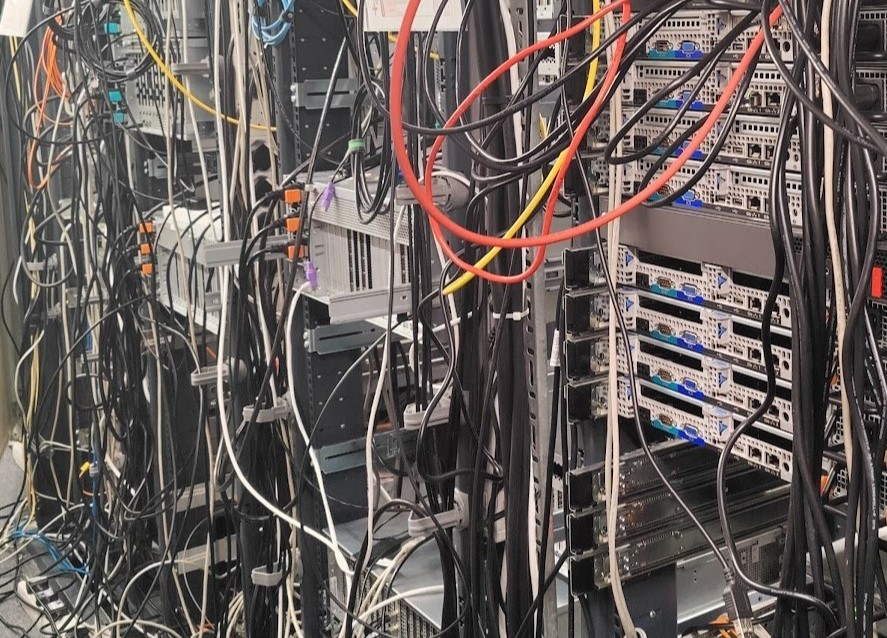
\includegraphics[width=0.40\linewidth]{images/server_racks.jpg}
    \caption{Server Rack within the school of Computer Science}
    \label{fig:server_rack}
\end{figure}

This is another reason that typical solutions cannot usually apply to these spaces, they are often designed for large data centres, where laptops can be used easily. For example, see below a photograph of the ideal system administrators setup. Where there is enough space to navigate between racks with a cart. In many scenarios, like that at Nottingham, this isn't an option. A tool that can be used on a mobile device in these less-than-ideal conditions has been something worthy of investigation. As mentioned the server space in Fig. \ref{fig:server_rack} is a good example. Before upgrades, the space was poorly lit and still is relatively cramped. It`s not particularly feasible to use a laptop in this space comfortably. But, as most alternative solutions assume the opposite and have cluttered user interfaces (UI), it makes certain tasks more difficult. The app provides a simplified, yet comprehensive interface to replace the need for a laptop in these situations.

Additionally the layout of servers and hardware shown above, made tracking cables completely impracticable and a mobile application has proved to be a great aid in the solution to this problem. Being able to see the configuration of a server in a visual way, in situ, has shown to be a great aid in the refactoring of the server space.

\begin{figure}[H]
    \centering
    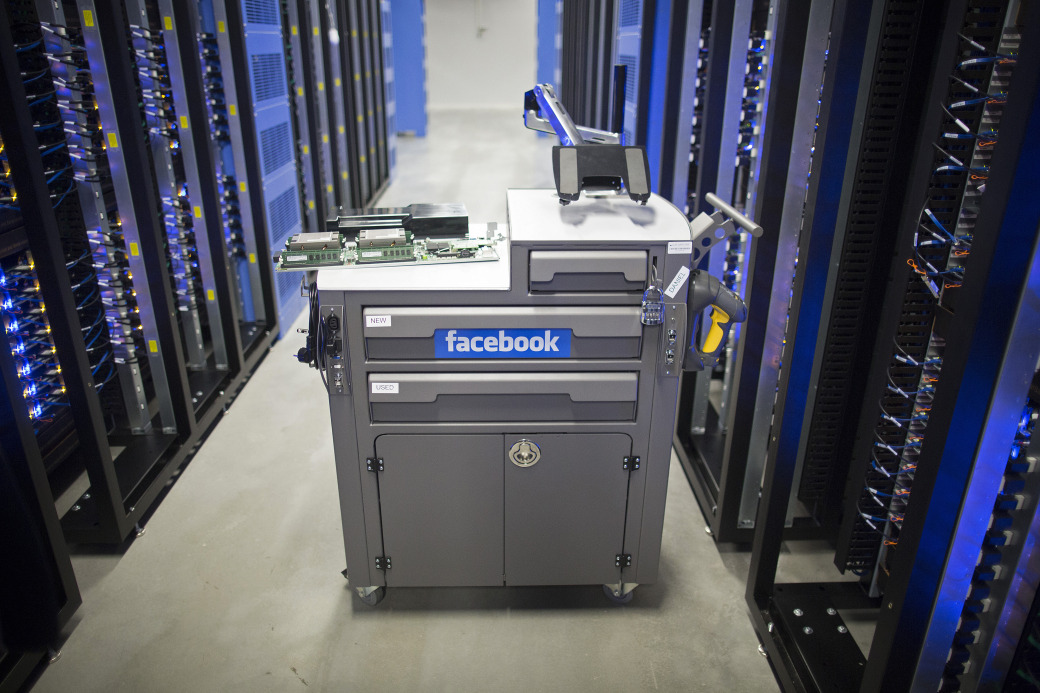
\includegraphics[width=0.42\linewidth]{images/facebook_cart.jpg}
    \caption{A more ideal administrator setup \cite{rosenblatt_2018}}
    \label{fig:_ideal_server_setup}
\end{figure}

Comparatively, another server space at Nottingham, that is focused on networking, shows a more realistic setup (\ref{fig:ideal_server_space}). Whilst the space is still cramped, the cable management is better and so the tracking of cables is more straight forward. Whilst this makes the task of tracing cables easier, it doesn't make the task of understanding the configuration of the server any easier. This is where software like netbox provides a source of knowledge that contains more information than a cable label can. But, critically the server space is still cramped and the use of a laptop is still impractical. The use of a mobile application is still a great aid in this situation.

\begin{figure}[H]
    \centering
    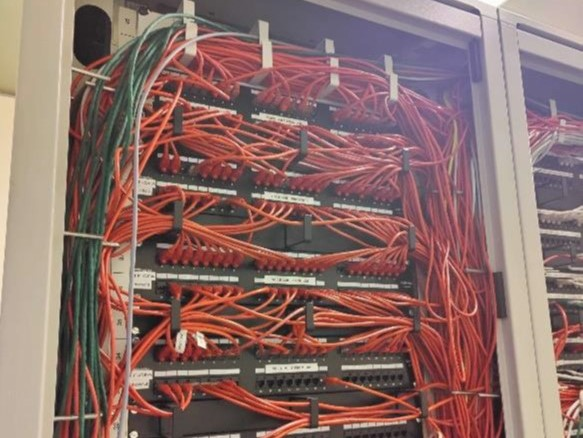
\includegraphics[width=0.43\linewidth]{images/server_racks_clean.jpg}
    \caption{More ideal and realistic server space}
    \label{fig:ideal_server_space}
\end{figure}


\subsection{Aims \& Objectives}
\label{sec:objectives}
The projects aims with their respective objectives.
\begin{enumerate} 
    
    \item[A1] To create a tool that will allow for cable configuration of server hardware to be
    easily digitised, visualised, queried and updated. 
        
    - To achieve this, the tool will integrated with Netbox, an open-source tool for managing network infrastructure. This will act as the backing database for the tool and will allow for the tool to be used in a wider context of server management.

        - The tool will use Netbox's API to query and update the database whilst using intuitive UI to allow for easy use.
        
        - To achieve visualisations, the tool will illustrate the cable connections between devices, showing data clearly and concisely.

    \item[A2] To create an in situ cross-platform mobile app that can be utilised in restricted
    spaces.    

    - To achieve this, the tool will be cross-platform and will be able to be used on any mobile device supported by the Flutter framework.
    
    - The tool will be designed with a focus on Human-Computer Interaction, to ensure that the tool is easy to use and can be understood by a wide range of users.

    \item[A3] To create an app that can interact with other open-source software easily
    
        - The tool will be open source, so modifications can be made to the tool to allow for it to be used in other contexts.
        
        - The tool will be built around modifiable models that can be changed easily for other software or a custom build backend.

\end{enumerate}

\subsection{Background}
\label{sec:background}
During my work for the Research Support Team and the challenges faced with server administration, I came to realise that there was a missing tool that could make a lot of tedious and time-consuming tasks easier. Once I began researching solutions to this, I came across Netbox, which is now our "source of truth" for our server space. It contains information about all of the hardware in the space, including the cables that connect them. Once Netbox began filling with data, the problem of finding and modifying that data in-situ arose. I found that using the full size interface was too clunky and so I wondered if there was a mobile app alternative, but there wasn't. This was the initial inspiration for the project. I wanted to create a tool that could be used in-situ, on a mobile device, to make the task of managing the server space easier. Whilst it can be appreciated that in large data centre applications, a mobile application like Keeptrack might not have the same desirability as a desktop application. But, acting as a companion tool alongside the desktop open-source software could be a great aid. With benefits for both platforms, they can be used in different situations, making workloads simpler and more efficient. Whilst there exists a companion app for a paid-for DCIM solution, there is no open-source equivalent. This was a gap in the market that the project aimed to fill, as well as carrying out research into the usage of mobile applications in this context.

\pagebreak

\section{Related Work}

In this section, three aspects of related work are discussed; existing applications similar to the project, related human-computer interaction research, and finally, papers related to technical aspects of the project.

\subsection{Application and Product Reviews}
\label{sec:app_reviews}

Following research on open-source and paid-for cable management/DCIM software, it was found there are limited options that have access to the trial versions without a legitimate business interest. This restricted the options of related applications that could be investigated. This aside, there follows three different software packages that are relevant to the project. Including; Sunbird DCIM\cite{Sunbird}, a paid-for solution with a trial accessible publicly. Next, Pathfinder Mobile \cite{Pathfinder}, a mobile counterpart to the enterprise "Pathfinder" package, was the only high-quality mobile solution that was discovered. Finally, Netbox \cite{Netbox}, the open-source DCIM software that the project will be built around. These three packages were shown to three individuals within the Research Support Team and their feedback was recorded. Each software was shown in mobile view. 

\subsubsection{Sunbird DCIM}
\label{sec:sunbird}
Sunbird DCIM is a feature-full Data Centre Infrastructure Management (DCIM) Package with a significant list of components. Their client list includes Paddypower, Betfair, eBay \& COMCAST \cite{Sunbird-we-know-data-centres}. When trialling dcTrack. their DCIM software, the immediate impression is that it is feature-rich, including monitoring environment, security, cooling as well as having asset and connectivity tracking. Whilst the server spaces within Computer science at UoN could benefit from a tool like this, its implementation and management would be quote the task. The tool is designed for large data centres and would be overkill for the server spaces within the school and other SMEs. For example, in fig \ref{fig:sunbird_dcTrack}, the space is approx 10x larger than that at Computer Science and this is one room in the example. 

\begin{figure}[H]
    \centering
    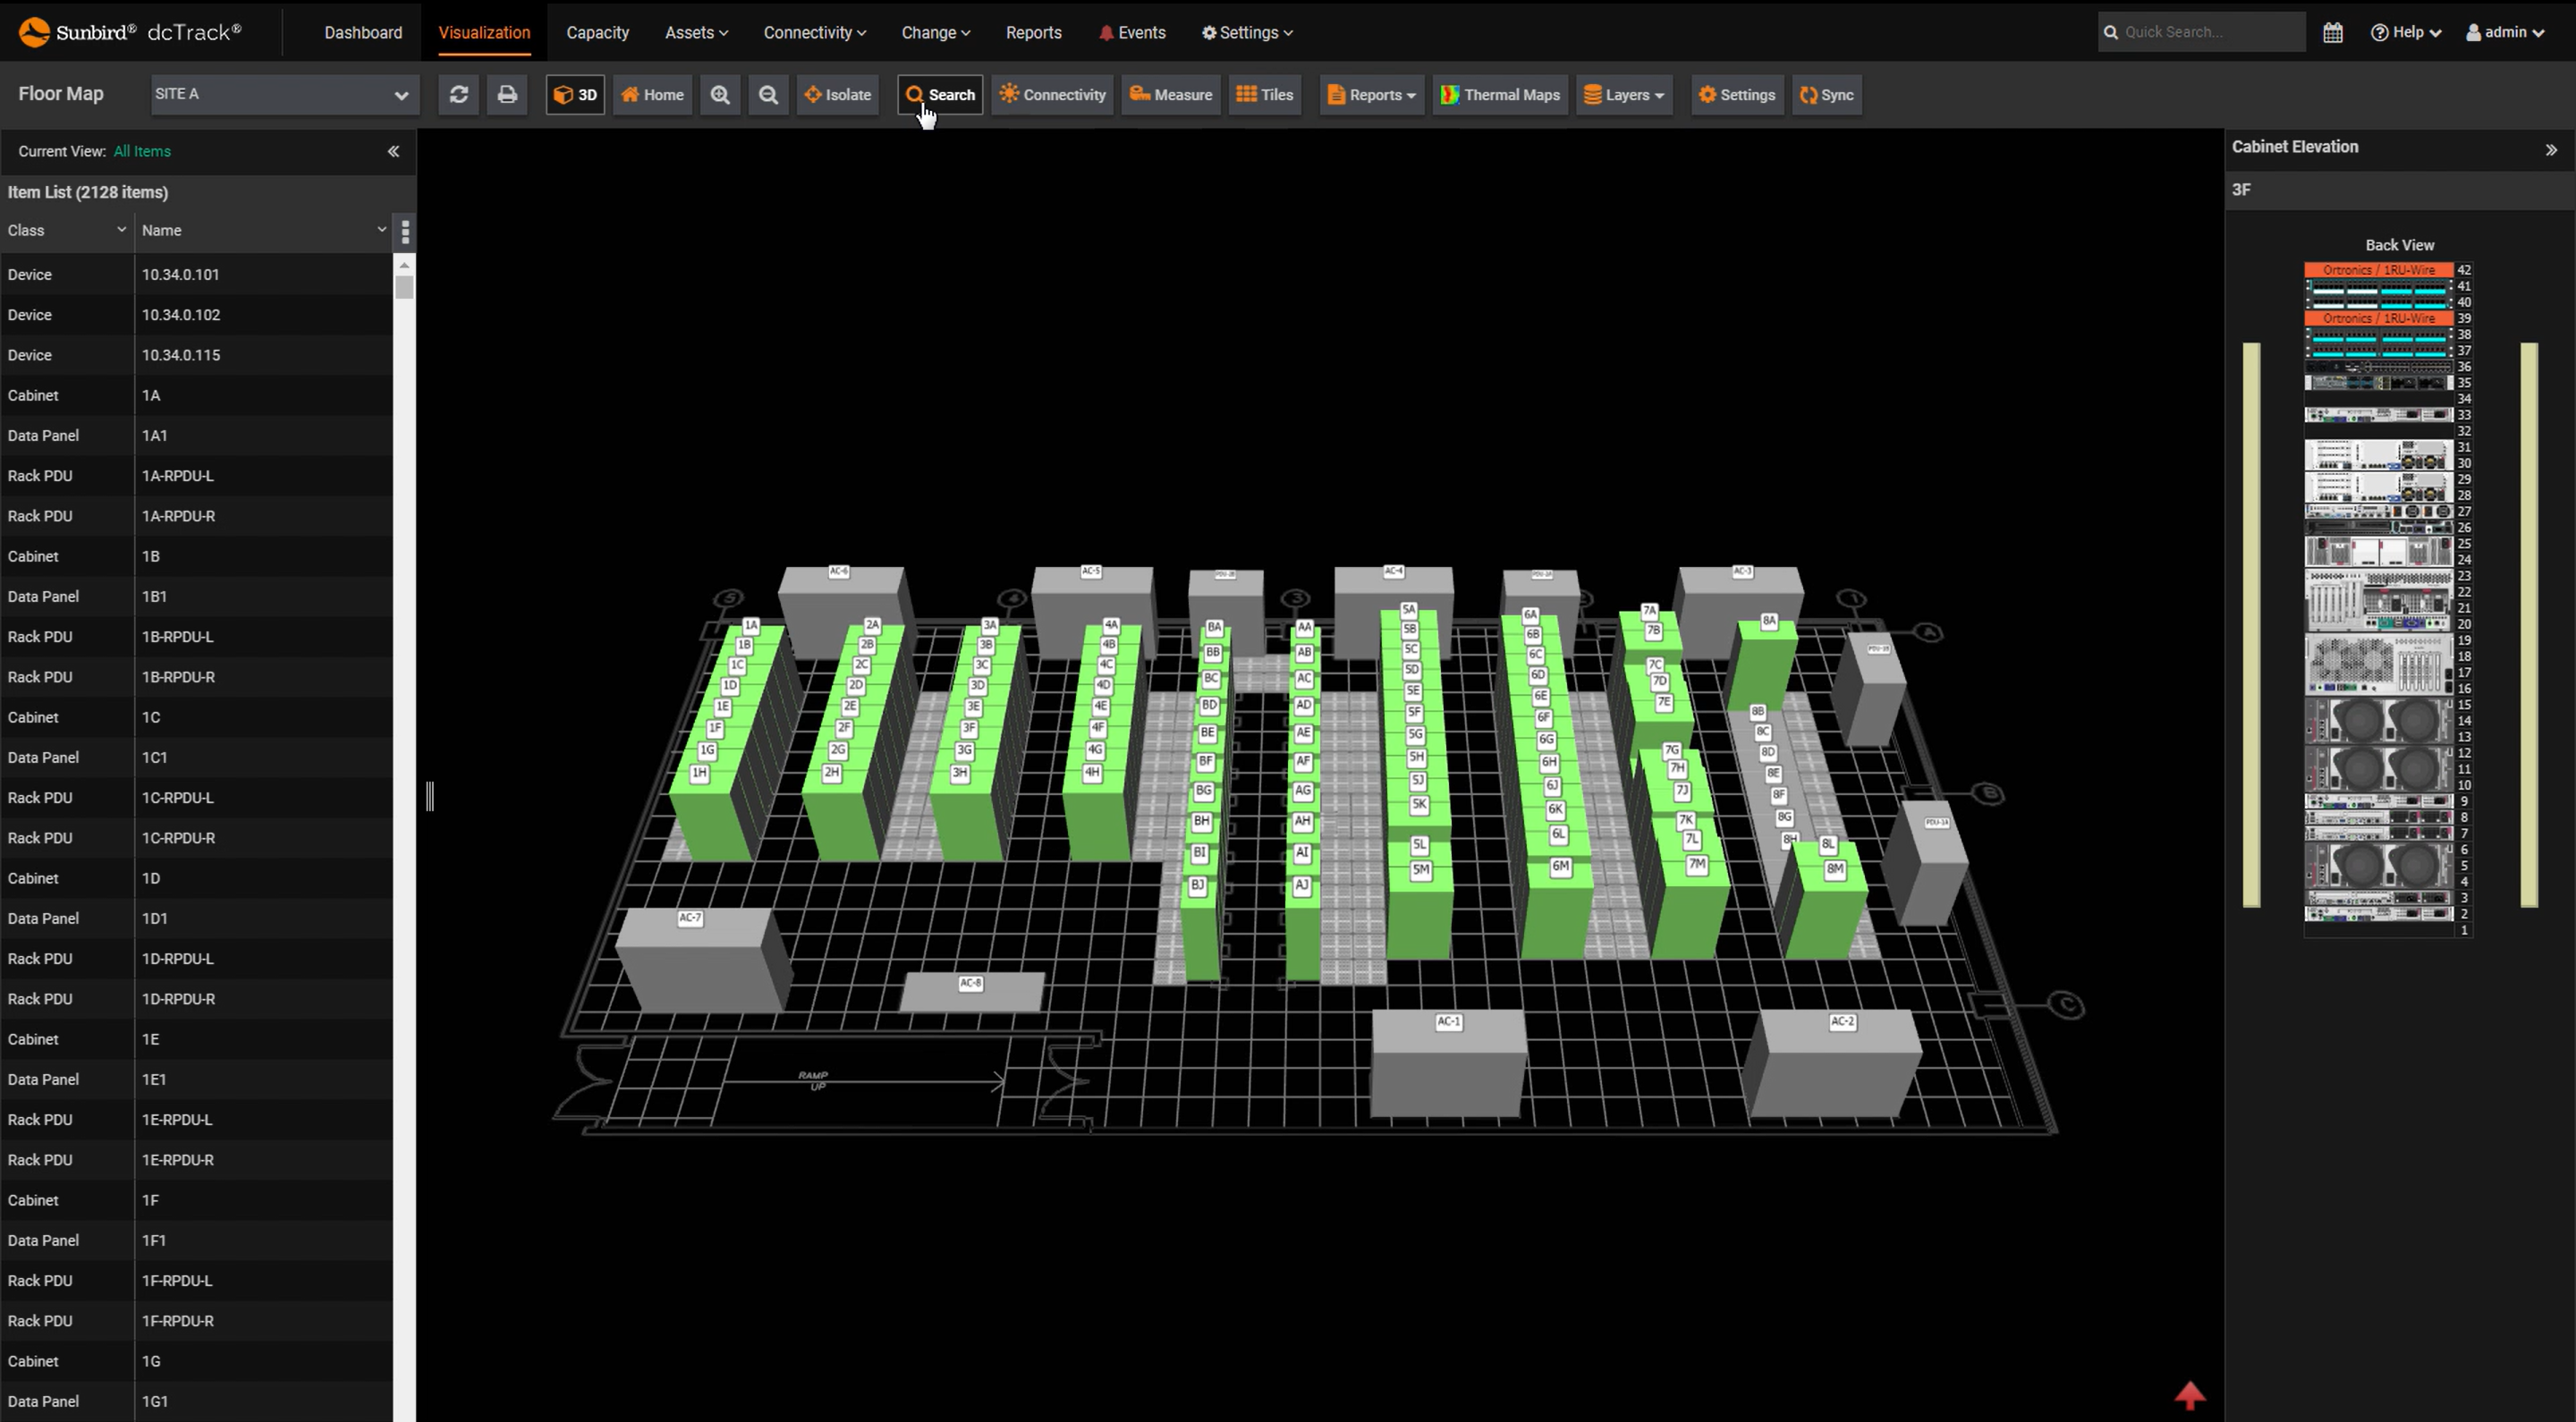
\includegraphics[width=0.8\linewidth]{images/sunbirddcim.png}
    \caption{Sunbird DCIM - dcTrack}
    \label{fig:sunbird_dcTrack}
\end{figure}

Though, some of its features could be useful in the implementation of the project. For example, the visualisation of data centres via a 3D model could be an interesting feature to implement in the project but might be out of scope. Especially with the additional research and testing that it would require. On the other hand, the search for assets and connections that Sunbird has, while thorough, is not as intuitive as the project aims to be. The immediate view lists all assets and their information, with 25 columns of data. It is overwhelming and not very useful without filters and custom views. Further, Sunbird intends to serve clients that might have thousands of assets, not quite hundreds like Computer Science has, so the requirements of searching and filtering are different. Though filtering by an extensive set of categories is a useful feature and could be implemented in the project, but in a more intuitive manner. 

% NOTE: Feature not implemented.

Sunbird is a prime example of what the project is not. It is enterprise-level DCIM software that is `overkill' for SMEs. Whilst it is a great tool for large data centres, its depth of features and complexity would add to the difficulty of implementing and using the software day to day.

\subsubsection{Pathfinder Mobile}
\label{sec:pathfinder}

Pathfinder Mobile is a mobile component to the complete Pathfinder package, it is designed to be used in conjunction with the full software and used as an "anytime and anywhere" \cite{PathfinderMobile} tool. It allows existing users of Pathfinder to access data remotely and in situ, with an intriguing focus on "work orders". These are created at a workstation, i.e. a laptop, which then synchronizes the work orders with the mobile app. From here the work orders can be executed on-site by using "graphical instructions support"\cite{Pathfinder}. Finally, on completion, all changes are uploaded to the pathfinder client. See below for screenshots from the Pathfinder Mobile app. 

\begin{figure}[H]%
    \centering
    \subfloat[\centering Side Panel]{{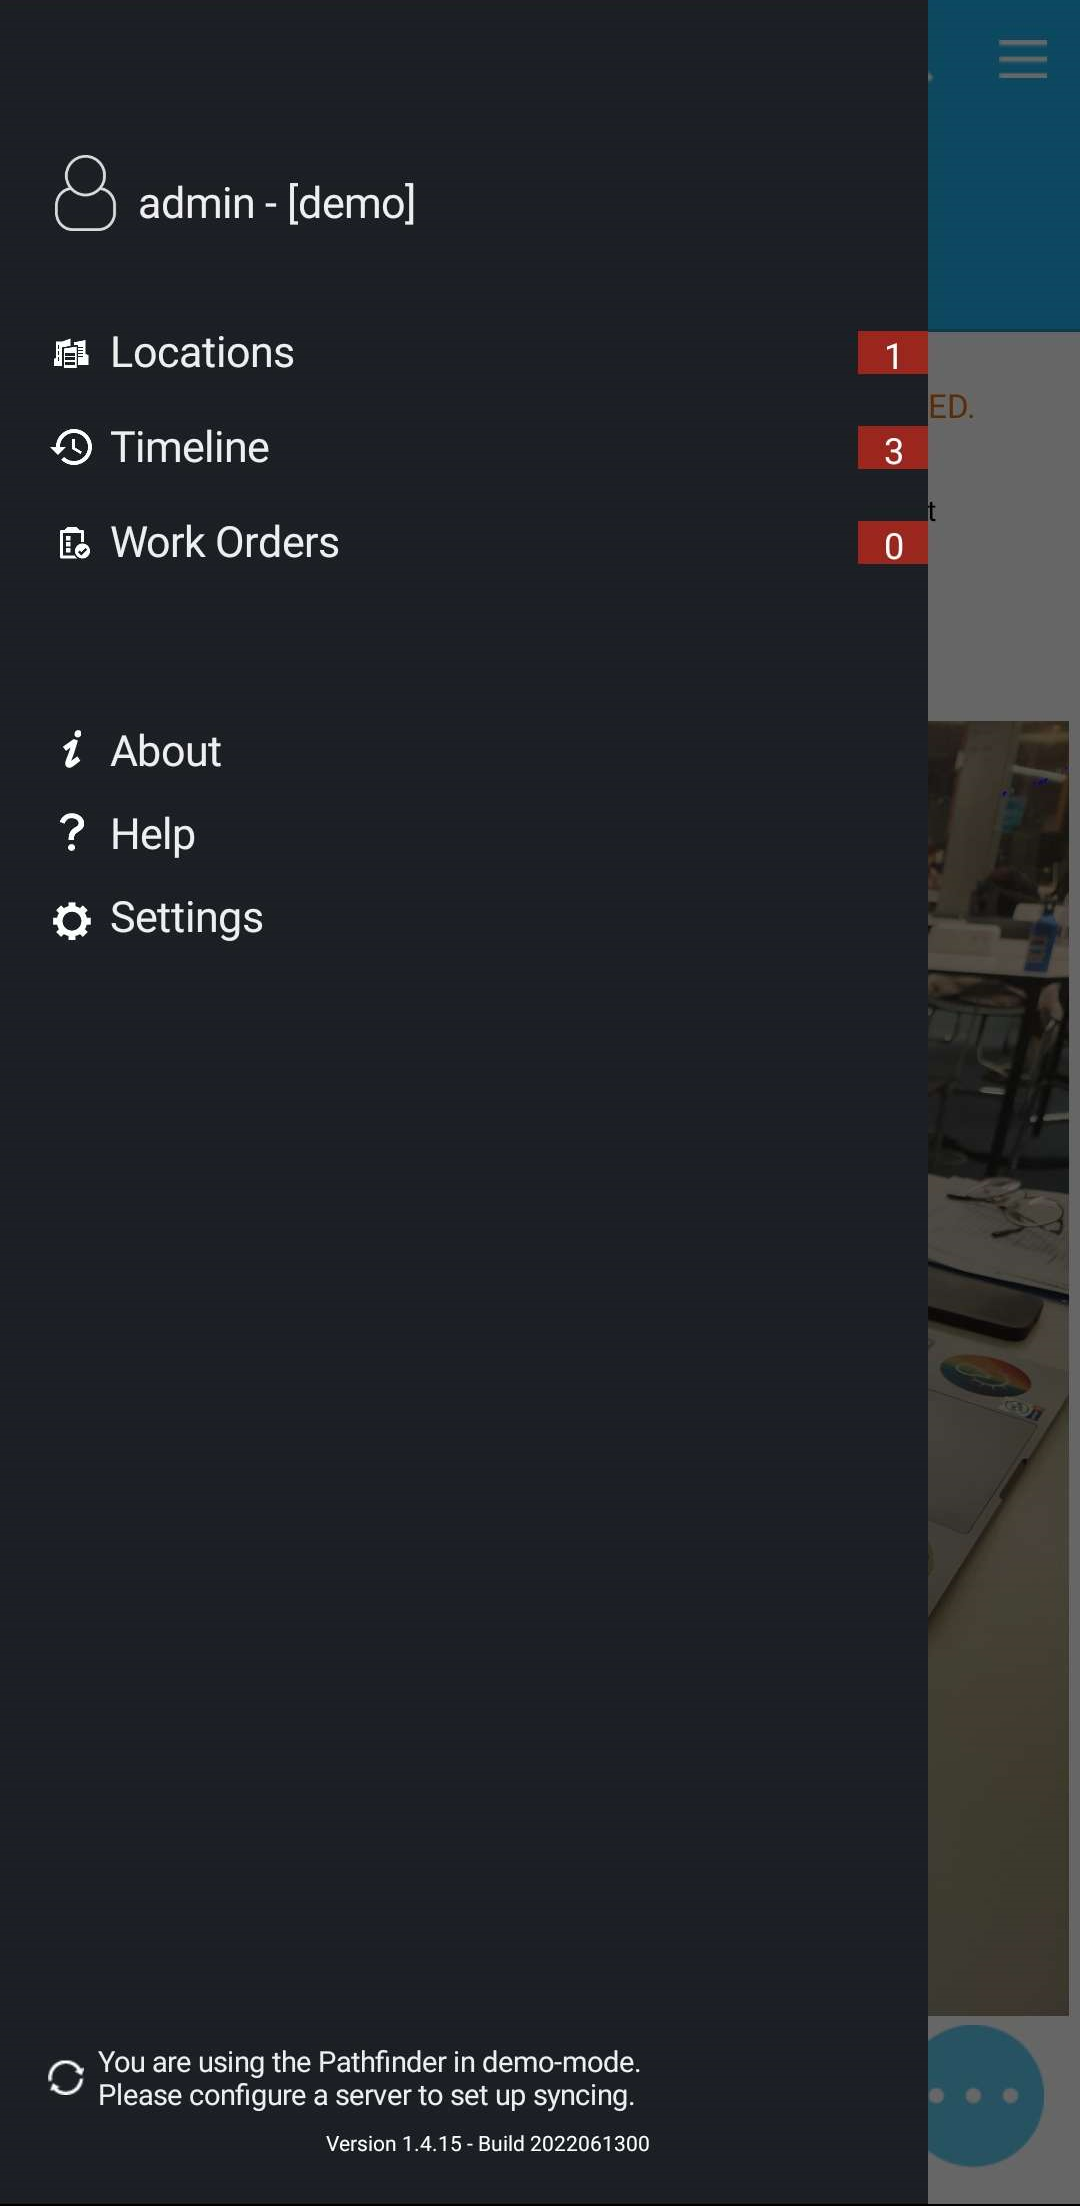
\includegraphics[width=4cm]{images/pathfinder_overview.png} }}%
    \qquad
    \subfloat[\centering Network Trace]{{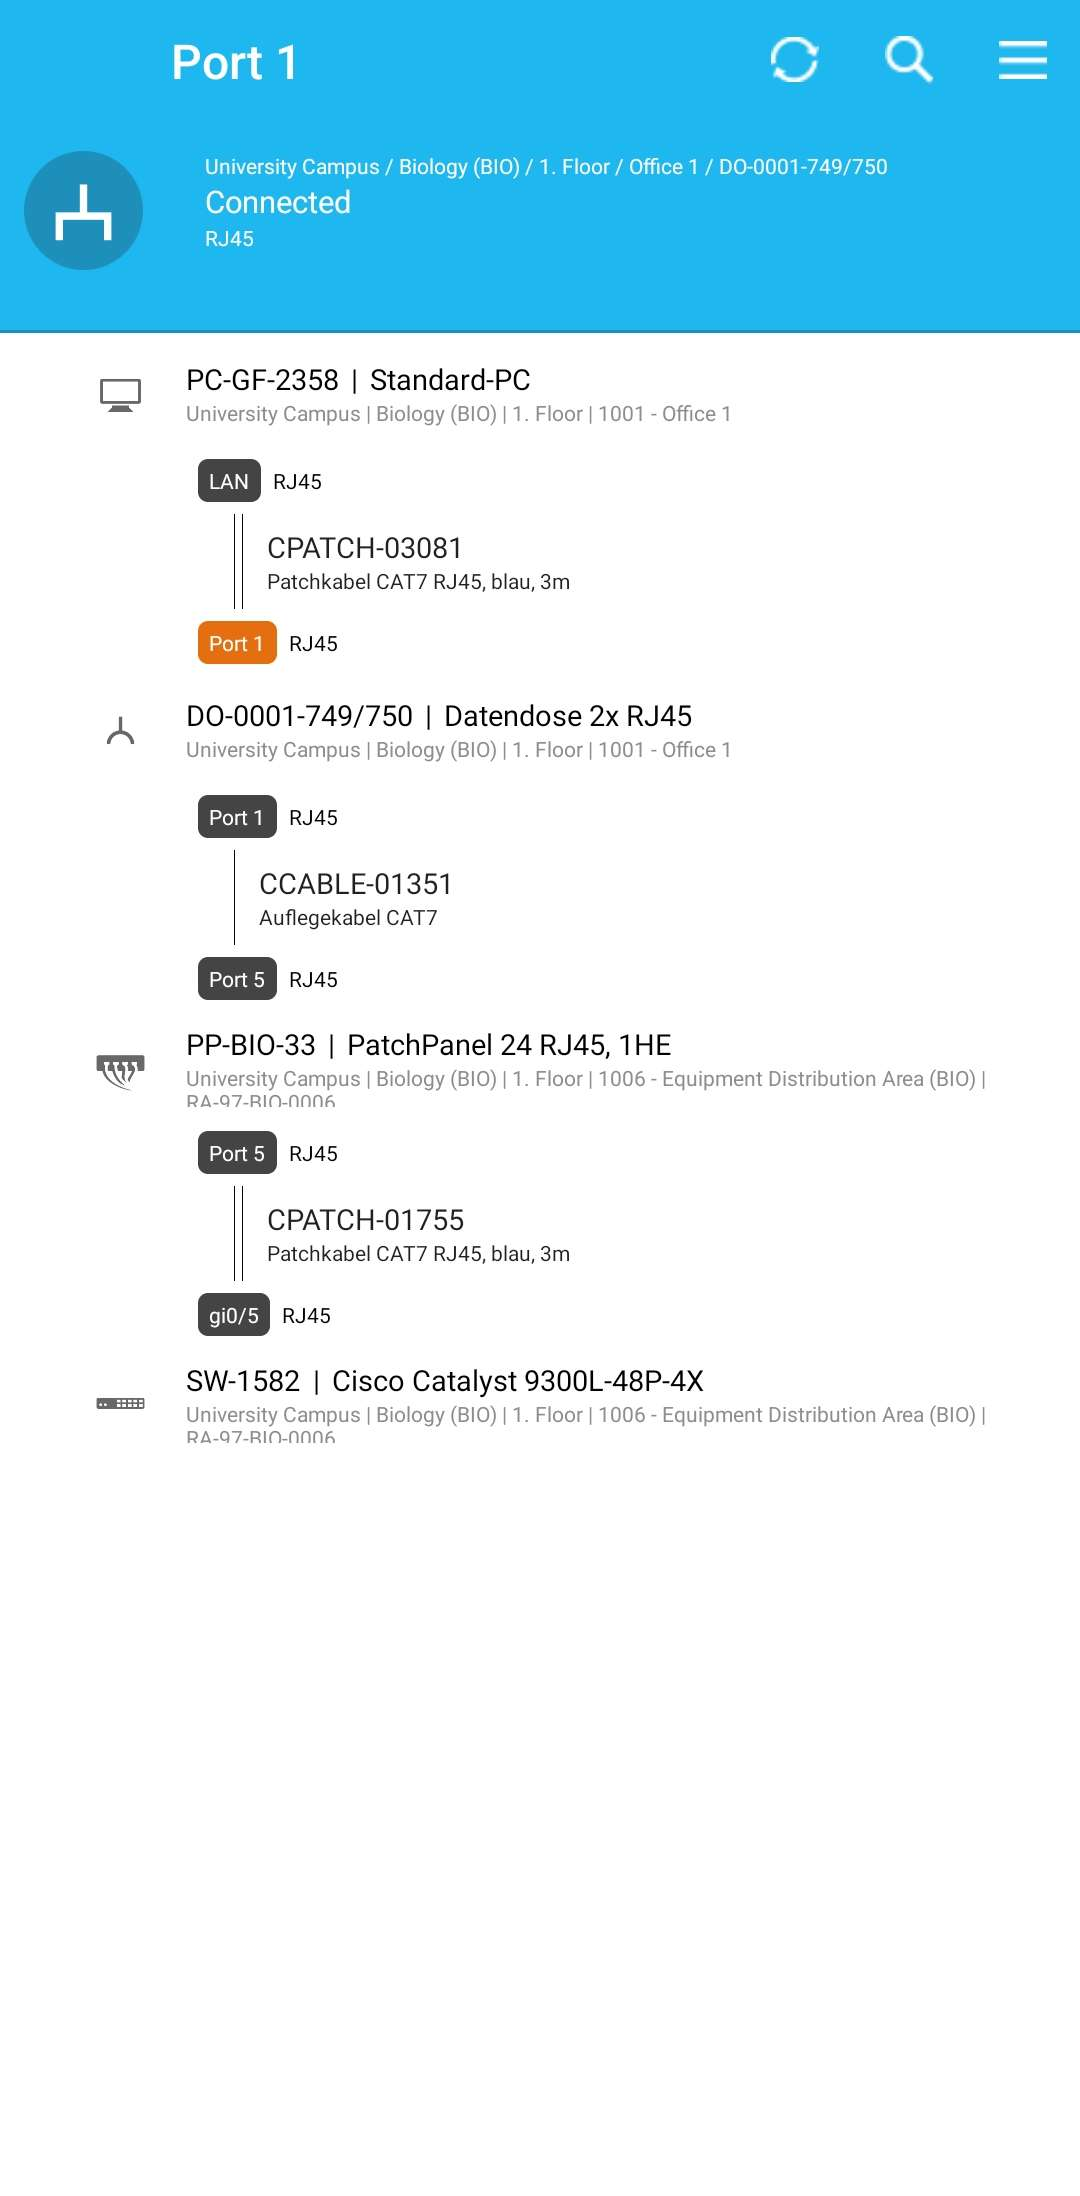
\includegraphics[width=4cm]{images/pathfinder_trace.png} }}%
    \caption{Screenshots of the Pathfinder Mobile App}%
    \label{fig:pathfinder_screenshots}%
\end{figure}

A similar environment interaction would work well for this project, with more complex modifications being completed/generated on a desktop client on the school's Netbox instance, i.e. templating. Then once completed, this can be synchronized with the mobile app to be used in situ. For example, verifying the correct cable is connected to the correct port. Additionally, completing work that is easier on desktop, e.g. adding a new asset, and then synchronizing it to the mobile app so that its networking configuration can be added in situ. 

The pathfinder app also allows for quick access to networking information, where users can complete the tracing of connections. Whilst this already was a core intention of the project, Pathfinders' method to visualise this is intuitive and similar to that which was discussed in the first Current State Analysis interview. These interviews are discussed more in detail in section \ref{sec:current_state_analysis}, but, notably, an interviewee mentioned a good method to do a visualisation is to list devices in a scrollable view. Then with each connection between them being drawn on the screen, along with device and interface information displayed as well. This is similar to the method used by Pathfinder, with; device name, location, interface name, type and cable type being displayed. This would aid in easing the process of tracing cables and connections, as well as verifying that the correct cable is connected to the correct port.

One aspect of Pathfinder that could be improved upon is the search functionality to find assets. Whilst they describe their search as being "text-rich". It seems to be less intuitive, and does a search based on every field, meaning that results for a simple search can be overwhelming. This is something that the project aims to improve upon, with a more practical search method, separating searches based on possible results. For example, not returning cables or power supplies when the user is only looking for devices. Further, their search by barcode scanner only simply enters the code into the search bar, not necessarily a bad method, but not as intuitive as it could be, for example - a button to scan the barcode, that on completion, automatically displays the asset information rather than needing another step.

A notable design element that the Pathfinder app implements is the focus on locations, assets, and connections in a hierarchical sense. For example, one method of displaying the data is to have a list of locations, then a list of assets within that location, and then a list of connections between those assets and so on. This is something that the project has also implemented due to the feedback from the interviews and has provided an straightforward way to display sometimes complex data.

Overall, Pathfinders mobile app has been a good reference point for the project. It has a similar focus and a similar method of visualising data. Though it is a companion of a larger software package that exceeds the current requirements of the school, it has features that has been referred to and implemented in the project.  

\subsubsection{Netbox}
\label{sec:netbox}
Whilst searching for a DCIM solution for the School of Computer Science, Netbox became a clear choice. It has a solid feature core, it's open source, self 'hostable' and can help solve the problems that the school is facing. As discovered during the Current State Analysis and personal experiences, the server rooms within CS are documented poorly due to a lack of consistent historical data. Most of the information is stored in the memory of long-gone staff or out-of-date spreadsheets. Netbox is to act as a "source of truth"\cite{Netbox}. More information on Netbox is included in the implementation section \ref{sec:development}. 

Netbox is built upon by several data models, which interact and are nestable with each other. For example, a device can be a child of a rack, which is a child of a site. This is a similar method to Pathfinder, and allows for a deeper relationship between data. This parent, child relationship allows for efficient tracing between devices and connections. With this approach and the solid API that Netbox provides it is possible to fetch this data and display it in a way that is intuitive and easy to use. One drawback of Netbox is the tracing of connections and addition of cables. It seems that the relationships can get a bit lost, and it is not as intuitive as it could be. This is something that the project improves upon, especially with in situ tracing, where navigating a large screen interface can be difficult. A primary example of this is the multiple type of port or interface that a device can have. For example, a switch can have console ports, power ports,  network ports, and management ports - All of which are displayed on different pages and can be nested within each other. It can be difficult to navigate this, especially when the device has a lot of ports. This is something that the project aimed to improve upon, with a more intuitive and efficient way to display this data.

Whilst Netbox is a great tool, it is not without its flaws. This projects solves one of its main issues, the clunky in situ use experience of the interface. Whilst it has a mobile friendly web interface, there are limits as to how friendly it can be. The limited screen retail needs to be used efficiently, and having a complex interface nested inside a browser app is not the best way to do this. Additionally, there is a lot of data to be loaded and displayed, in a browser this can show as loading bars and low frame rate. Here is where Keeptrack comes in, to sit on top of Netbox and provide a more intuitive and efficient interface for the user.  


\subsection{Papers focused on HCI and User Experience}
\label{sec:HCI}
There is a lack of significant research into areas of Human-Computer Interaction and User Experience in the context of server management. But for the few papers that are relevant to the project, they have aided in its development. The first paper is a write-up by Yin et al. \cite{cloud3dview} regarding their demonstration of Cloud3DView at SIGCOMM '13. Cloud3DView is an interactive 3D visualisation tool used for cloud focused data centers. It uses FPS gamification to allow users to monitor situations and visualise data from a user-friendly interface, all remotely. Cloud3DView also included a focus on its use of "cutting-edge HCI technologies" \cite{cloud3dview}. Whilst the paper itself doesn't go into the reasoning of why certain HCI choices were made, it shows a good example of how a mobile device can be used to interact with a data centre and can be used to improve efficiency and user experience. Though the focus of this project isn't to be a 3D visualisation tool, one aspect of Cloud3DView is the ability to view data about the devices in a 3D environment. Whilst, a 3D visualisation is out of scope for KeepTrack, an augmented reality feature was considered to be implemented and was discussed in the Current State Analysis interviews. This feature would allow users to view data/connections concerning the devices via a camera on their mobile device, offering an alternative method of visualisation. Though, in order to implement this, significant research would need to be done into the best way to implement this feature and how it would interact with the server room environment.

Notably, in the paper about Cloud3DView, there was a focus on using mobile devices to be used for data visualisation, but no mention about the their possible use for data entry. With the nature of the data being entered in server management, in some cases a mobile format may offer a more intuitive/accessible platform than a desktop device. For example, entering the connection between two assets, where the information can be verified in situ in real time versus sat at a desk far away. This is one of the work flows that the project was developed to improve upon.

An important benefit of using mobile devices for data entry is the ability to use multiple interface types to enter data. For example, a user can enter data via an alphanumeric keyboard, numerical keypad, calendar picker, lists etc all whilst benefiting from the ease of a touch screen interface. A comparative analysis into different data entry design patterns investigated three different patterns for seven different data types for a set of nine tasks testing different patterns \cite{myka2019comparative}. The investigation completed a set of usability tests to determine which pattern was the most effective, with different patterns benefiting different tasks/data types better than others. The results from this study will be used to inform the design of the interface for the project. Specifically for this project, the most relevant data types are; small numbers, single-choice lists and text.

On a similar note, a study into the structure of data entry on mobile devices noted that existing interfaces "interfere with user input" and force "complex interactions to enter simple information" \cite{van2007gui}. This is especially apparent in some cases of the Netbox interface e.g., as mentioned previously, adding cable connections. Whilst, naturally, there are limitations as to how streamlined an interface can be on a desktop-based web application, there is more room for improvement on a mobile application. For example, the addition of a cable on mobile can be reduced to far fewer steps than on the web interface. Whilst it might reduce the granularity of the data, it would be a trade-off that would be worth it for the ease of use. Additionally, the project aimed to improve upon the current interface, not replace it. The current interface will, in theory, still be available for users who prefer it, or for more complex tasks.

Kleek et al's \cite{van2007gui} study further focused on the structure of data entry on mobile devices, its importance, but also the importance of not creating interfaces that deter users from entering data. Highlighting a fine balance between the two. One of the sources of problems for the school is the lack of data ever being entered anywhere. If the project has an interface that dissuades users or is perceived as too tedious then it will not solve a key problem. This project took upon the findings of this study to ensure that the interface is intuitive and easy to use. For example, an automatic filtering search bar for assets and replacing text fields with barcode scanners or other input methods.

\subsection{Papers focused on Technical aspects of the project}
\label{sec:technical}

One key part that the project aimed to improve is the searchability of assets, i.e. finding the asset desired quickly and accurately through many means. The current method of asset identification is inconsistent with different naming conventions, ID codes, labels, no labels, hostnames etc. The Centre for the Protection of National Infrastructure (CPNI) produced a paper on the importance of asset management, specifying that, "all organisational assets and systems that are necessary for the delivery of effective operations or are of specific organisational value, should be identified." \cite{cpni}.

Not only is it important to identify assets whilst they are in use, but also for documenting any changes, journal entries, ownership, location etc. This project also aimed to improve upon this, with a focus on the identification of assets being homogenous and consistent. Keeptrack uses the netbox model IDs as a unique identifier for each asset, cable and interface. This way, they can be referred to individually and updated in a consistent manner. 

In this project, assets are considered to be both physical server hardware, such as servers, switches, KVM`s, NAT etc. but also cabling, such as ethernet, fibre, SFP and power. To identify each of these assets uniquely it was decided that an encoded label would be best. A comparative study into barcodes, QR-codes and RFID systems in the library environment looked into the respective advantages and disadvantages of each \cite{lotlikar2013comparative}. Going by these attributes, it is more sensible to use Barcodes or QR codes for the project. With RFID tags being more expensive, as well having a higher risk of tag collisions. This occurs when many tags are in close proximity\cite{lotlikar2013comparative}, like that of a server room, and a reader misreads their value to be another. An issue like this would likely add to the time-consuming tasks and make for a more frustrating workflow. Further, a specialised reader is likely needed and so another handheld device would need to accompany the app.

Additionally, a paper written on the review of QR codes highlights that QR codes can store more data in the same area, have data redundancy, are faster to scan and are "readable from any direction in 360\degree"\cite{mishra2017review}. Whilst these benefits seem to make it the clear choice over barcodes, QR codes contain data in both dimensions. Though this is a benefit in most use cases, it is likely to pose a problem when scanning codes stuck to ethernet cables.

Where, barcodes contain data in one dimension which is then repeated vertically, allowing for their placement to be more dynamic, e.g. on a cable. This is clearly shown in figure 3 of Mishra et al., fig. \ref{fig:barcode}. So, for this project it was initially decided that it will use barcodes for cables, and then QR codes for other assets will be used. But after the interview processes and observations, it was decided that QR codes would be more beneficial as they can store more contextual data. It was realised following consultation from CGI, the global IT consultation firm, that having labels that only hold abstract data can be considered a single point of failure to gather information. Especially as it was initially decided that the information stored for cables will be a random short number assigned to each cable, suitable for barcodes - But completely abstract for humans to read. So in the situation of netbox being down, or the QR code being damaged, the information stored on the label would be useless. Therefordde a combination of a meaningful label and a QR code would be used. Then each QR code will store the netbox unique ID for that cable. This way, the QR code can be scanned and the information can be retrieved from netbox. This is a more robust system than just having a label with a randomly generated number.

\begin{figure}[H]
\centering
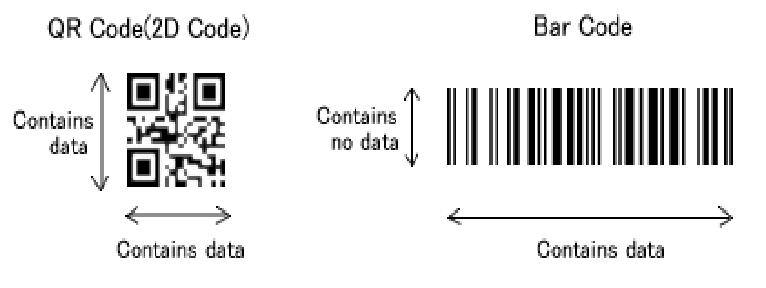
\includegraphics[width=.75\textwidth]{images/barcode_mishra.png}
\caption{Barcode vs QR code}
\label{fig:barcode}
\end{figure}

Whilst an Augmented Reality visualisation feature is dependent on time and the success of other elements. It is still important to consider related work with these features, especially as it could be a feature added on. Whilst already investigating Cloud3DView \cite{cloud3dview}, which uses 3D visualisation, a more apt implementation would be by using the QR codes placed on assets to aid in visualising data. This is very similar to the work outlined in the paper, "Applying QR code in augmented reality applications" \cite{applyingQR}. This paper displays how the elements of the QR code can be used to position elements in the AR scene and simultaneously generate information embedded in the QR code. Should this be a feature that can be implemented, it is likely the project will follow a similar method as to what Kan et al. set out \cite{applyingQR}. With the existing desire to implement a multi-format code scanner, i.e. both barcode and QR, this would be a good addition to the project. Further, there already exists a cross-platform plugin for Augmented Reality in Flutter which can be utilised \cite{ar_flutter}.

\section{Description of the Work}
\label{sec:work}
This project aims to create a mobile application that will allow users to add, view and manage assets and cables in server rooms. With the specific application to Small/Medium enterprises. The application will be built using Flutter, a cross-platform framework which will allow for the app to be used on both Android and iOS devices. The application will be built upon Netbox DCIM \cite{Netbox} and their RESTful API \cite{NetboxAPI}. 

The project aims to build upon this API to create a more user-friendly and intuitive interface for server administrators to use. With this in mind, a second key aspect is investigating the best interface for data entry in this context. This will be done by interviewing and observing the system administrators at the school using iterative prototypes of increasing fidelity.

\subsection{Project Stretch Goals}
\label{sec:stretchgoals}
Following the interviews during the current state analysis and the investigation of similar work, the further goal to implement an augmented reality visualisation feature is desirable. This feature will allow users to visualise asset information and networking details in a highly interactive way. 

Desirable features that could be implemented depending on time constraints in priority order: 
\begin{itemize}
\item Journals for assets, allowing for notes to be added to assets, e.g. when a new component is added, or when a component is removed.

\item Auditing of assets, allowing for the user to scan an asset and then be presented with a form to fill out, e.g. the asset is in good condition, or the asset is faulty. 

\item In-App SSH terminal, allowing for the user to connect to a device and run commands, e.g. to check the status of a service.

\item Augmented reality to visualise asset information and networking details.
\end{itemize}

\section{Methodology}
\label{sec:methodology}
With all of the aims and aspects of the projects in mind, it was decided to use a participatory design approach, with iterative prototypes of increasing fidelity. Then, with user evaluation and feedback, the final product will be created. This will be done by following the steps outlined in the following list:

\begin{enumerate}
    \item Create low-fidelity prototypes
    \item Current state analysis and initial interviews
    \item Create higher fidelity interactive prototypes
    \item User evaluation and feedback
    \item Minimal Viable Prototype with user feedback
    \item Create final product
\end{enumerate}

Whilst deciding on a cross-platform framework to build this project on, Flutter become the obvious choice. Not only with previous experiences working with it, but also with the fact it has become the most popular cross-platform framework \cite{JetBrainsFlutter}. Further, with personal work in aiding the development of Labmonitor\cite{labmonitor}, there is a familiarity with the code scanning package that will also be used in this project\cite{barcodeScannerPlugin}.

\subsection{Current State Analysis and Initial Interviews}
\label{sec:current_state_analysis}
To begin with, using personal experience, knowledge and  understanding of the requirements, a set of low-fidelity prototypes were made. These were primarily created in order establish an initial set of features. A set of interviews were conducted with the system administrators (RST) to extend upon original experiences.  Within these interviews, the current state of the system was discussed, to understand the current workflow and the problems that are faced.

This was done by asking broad questions such as:

\begin{itemize}
    \item What are your opinions on the current state of the server room?
    \item What do you think could be improved?
    \item Do you have any suggestions for the new system?
\end{itemize}

Then, each interviewee was showed the low-fidelity prototype of the application, intending to gather initial thoughts on the proposed layouts and to see if there were any features that they would like to see added/removed. Their responses were recorded and then analysed, to identify any repeating ideas, mainly using thematic analysis \cite{thematicAnal}.

\section{Design}
\label{sec:design}
The following section will outline the design of the project. Specifically; the user interfaces design, the system architecture and the interviews and observations that have been conducted.

\subsection{User Interface Design}
\label{sec:ui_design}
Following the initial interviews, a set of high-fidelity prototypes are being created. These are currently being created using Figma \cite{figma}, a web-based prototyping tool. Chosen due to extensive prior use and its high reputability, with the UX Design Institute describing it as the best prototyping tool \cite{figmaUX}. With Figma's prototyping features, it is possible to create interactive prototypes, these will then be used to conduct further interviews, but with a more evaluative, task-based, focus. Then based on the feedback, an initial Minimal Viable Product (MVP) will be created. This will be done by following the steps outlined in the next section. Then an evaluation will be made on the MVP, to inspire any last changes/features in the final design, which then will be used to build upon the MVP to create the final product. See below for the current high-fidelity prototype progress.

\begin{figure}[H]
    \centering
    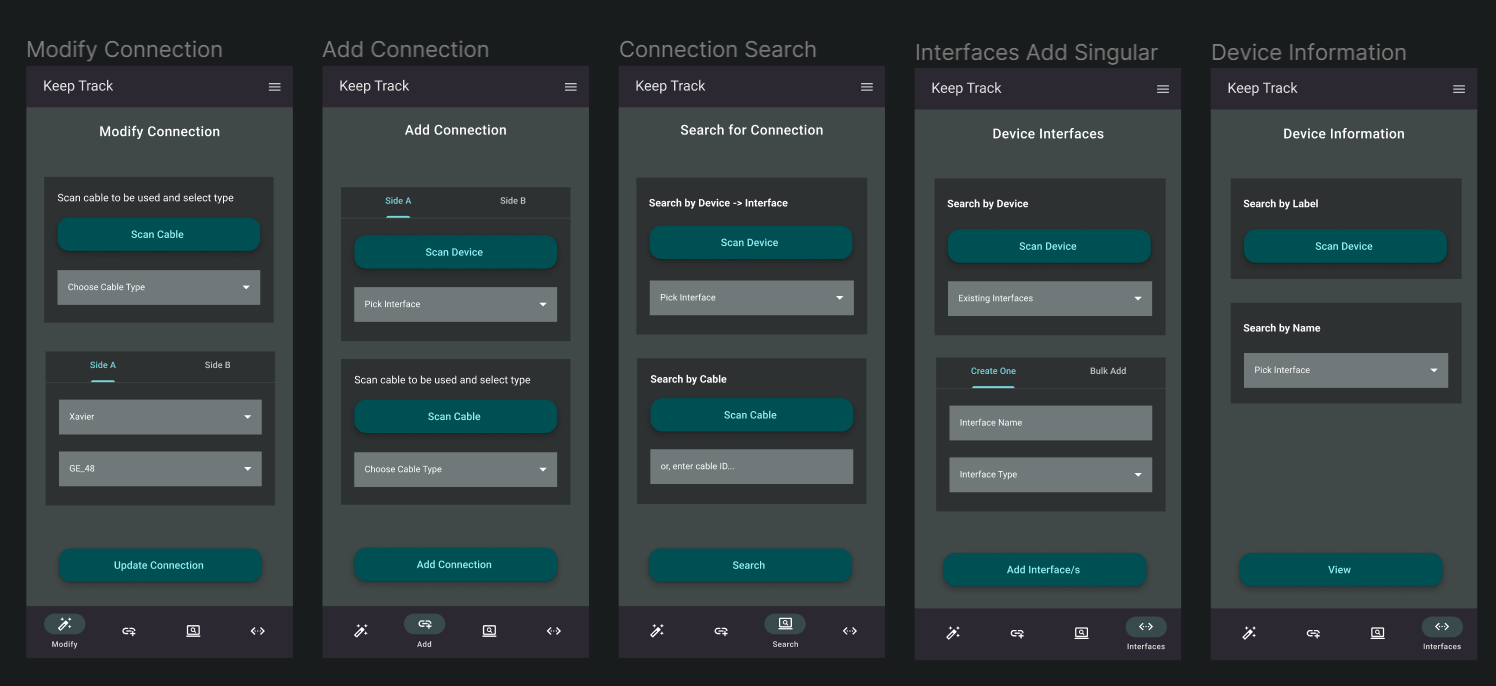
\includegraphics[width=1\textwidth]{images/figma_prototype.png}
    \caption{Figma Prototype}
    \label{fig:figma}
\end{figure}


The interface will be based on the Material Design, which is described as "an adaptable system of guidelines, components, and tools that support the best practices of user interface design."\cite{materialDesign}. It has several User Experience (UX) principles at its core (such as accessibility) that will create a user-friendly interface. Material is widely used and will give users a sense of familiarity, especially icons and GUI elements. This similarity will increase learnability and reduce the user's cognitive load.

\subsection{Development and System Architecture}
\label{sec:development} 
For the development of the app, as mentioned and reasoned in section \ref{sec:technical}, Flutter will be used to create the app. The following diagram describes how the app will interact with the Netbox Instance using its REST API. These calls are processed through NGINX which is working as a reverse proxy.

\begin{figure}[H]
    \centering
    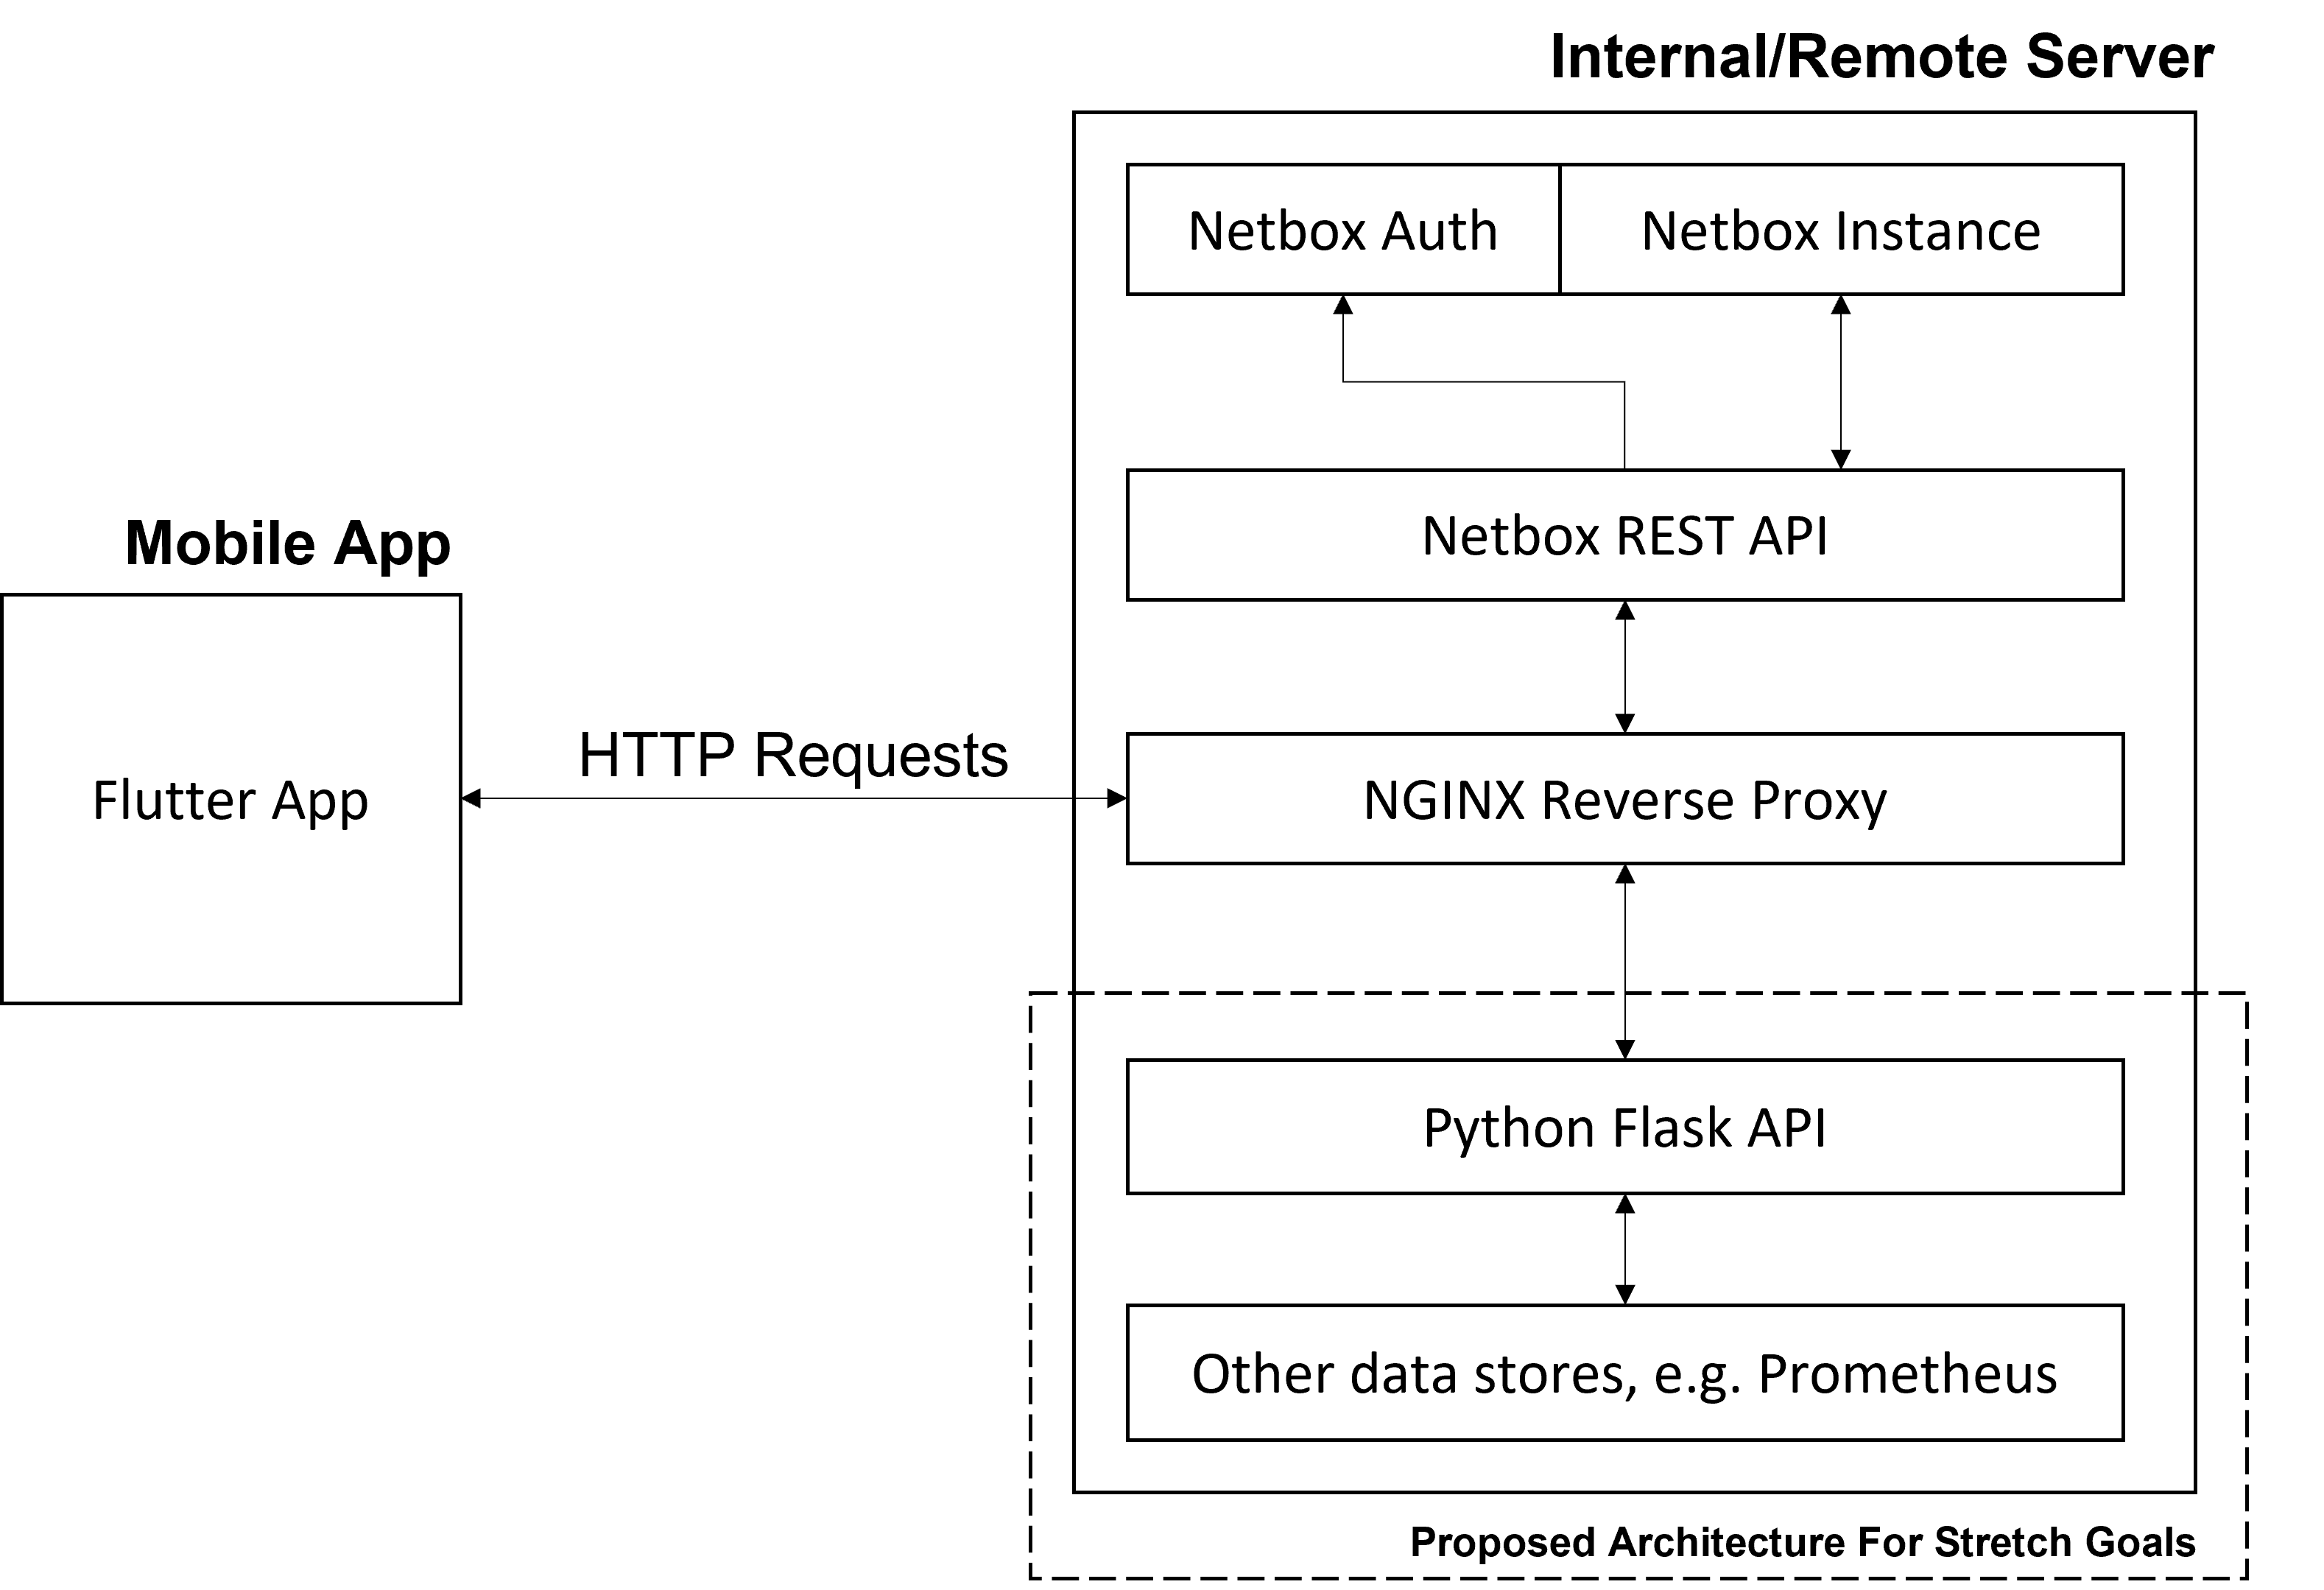
\includegraphics[width=0.6\textwidth]{images/top-level-archi.png}
    \caption{System Architecture}
    \label{fig:architecture}
\end{figure}

The app will use Netbox's inbuilt Django user authentication system, which allows for tokens to be created via an API call. This token will then be used to authenticate the user to fetch data and make changes to the Netbox instance, returning any errors should a permission problem arise. For stretch goals, should the app feature more information or processing, the requests will still go through the same NGINX reverse proxy but to a different API endpoint. Though open to change, a Python-based Flask Server will be used to handle requests external to Netbox. 

The app will be structured using a Data Access Object (DAO) pattern\cite{dao}, to separate the data access from the logic. In a way, replicating the data objects within Netbox itself. This will allow for the app to be easily extended and modified in the future. 

Further, there is a separation between views, API calls and providers. This gives a more modular structure and provides more maintainable code, especially as requirements change, or Netbox updates/changes. Additionally, in the spirit of Open Source Software, the code will be stored on GitHub \cite{keeptrackgithub} and will utilise environment variables to store sensitive information so that other developers can easily implement their instance of the app.

\section{Implementation}
\label{sec:implementation}
The implementation has focused on the development of the core logical structure of the app and the creation of a foundation for the UI to test functionality. The current progress allows a user to sign into the app using their Netbox credentials. This information is then stored securely using the Flutter Secure Storage plugin \cite{securestorage}. The current UI allows the user to add a connection between two devices. More specifically, it allows searching for devices via a searchable dropdown, which then dynamically loads its interfaces, with a tab view that allows the user to select the interface on each device. Further, the current implementation has a working integration of the barcode/QR code scanner plugin \cite{barcodeScannerPlugin}. See below for screenshots of the current UI, fig. \ref{fig:currentUIScreenshots}. 

\begin{figure}[H]%
    \centering
    \subfloat[\centering Login Page]{{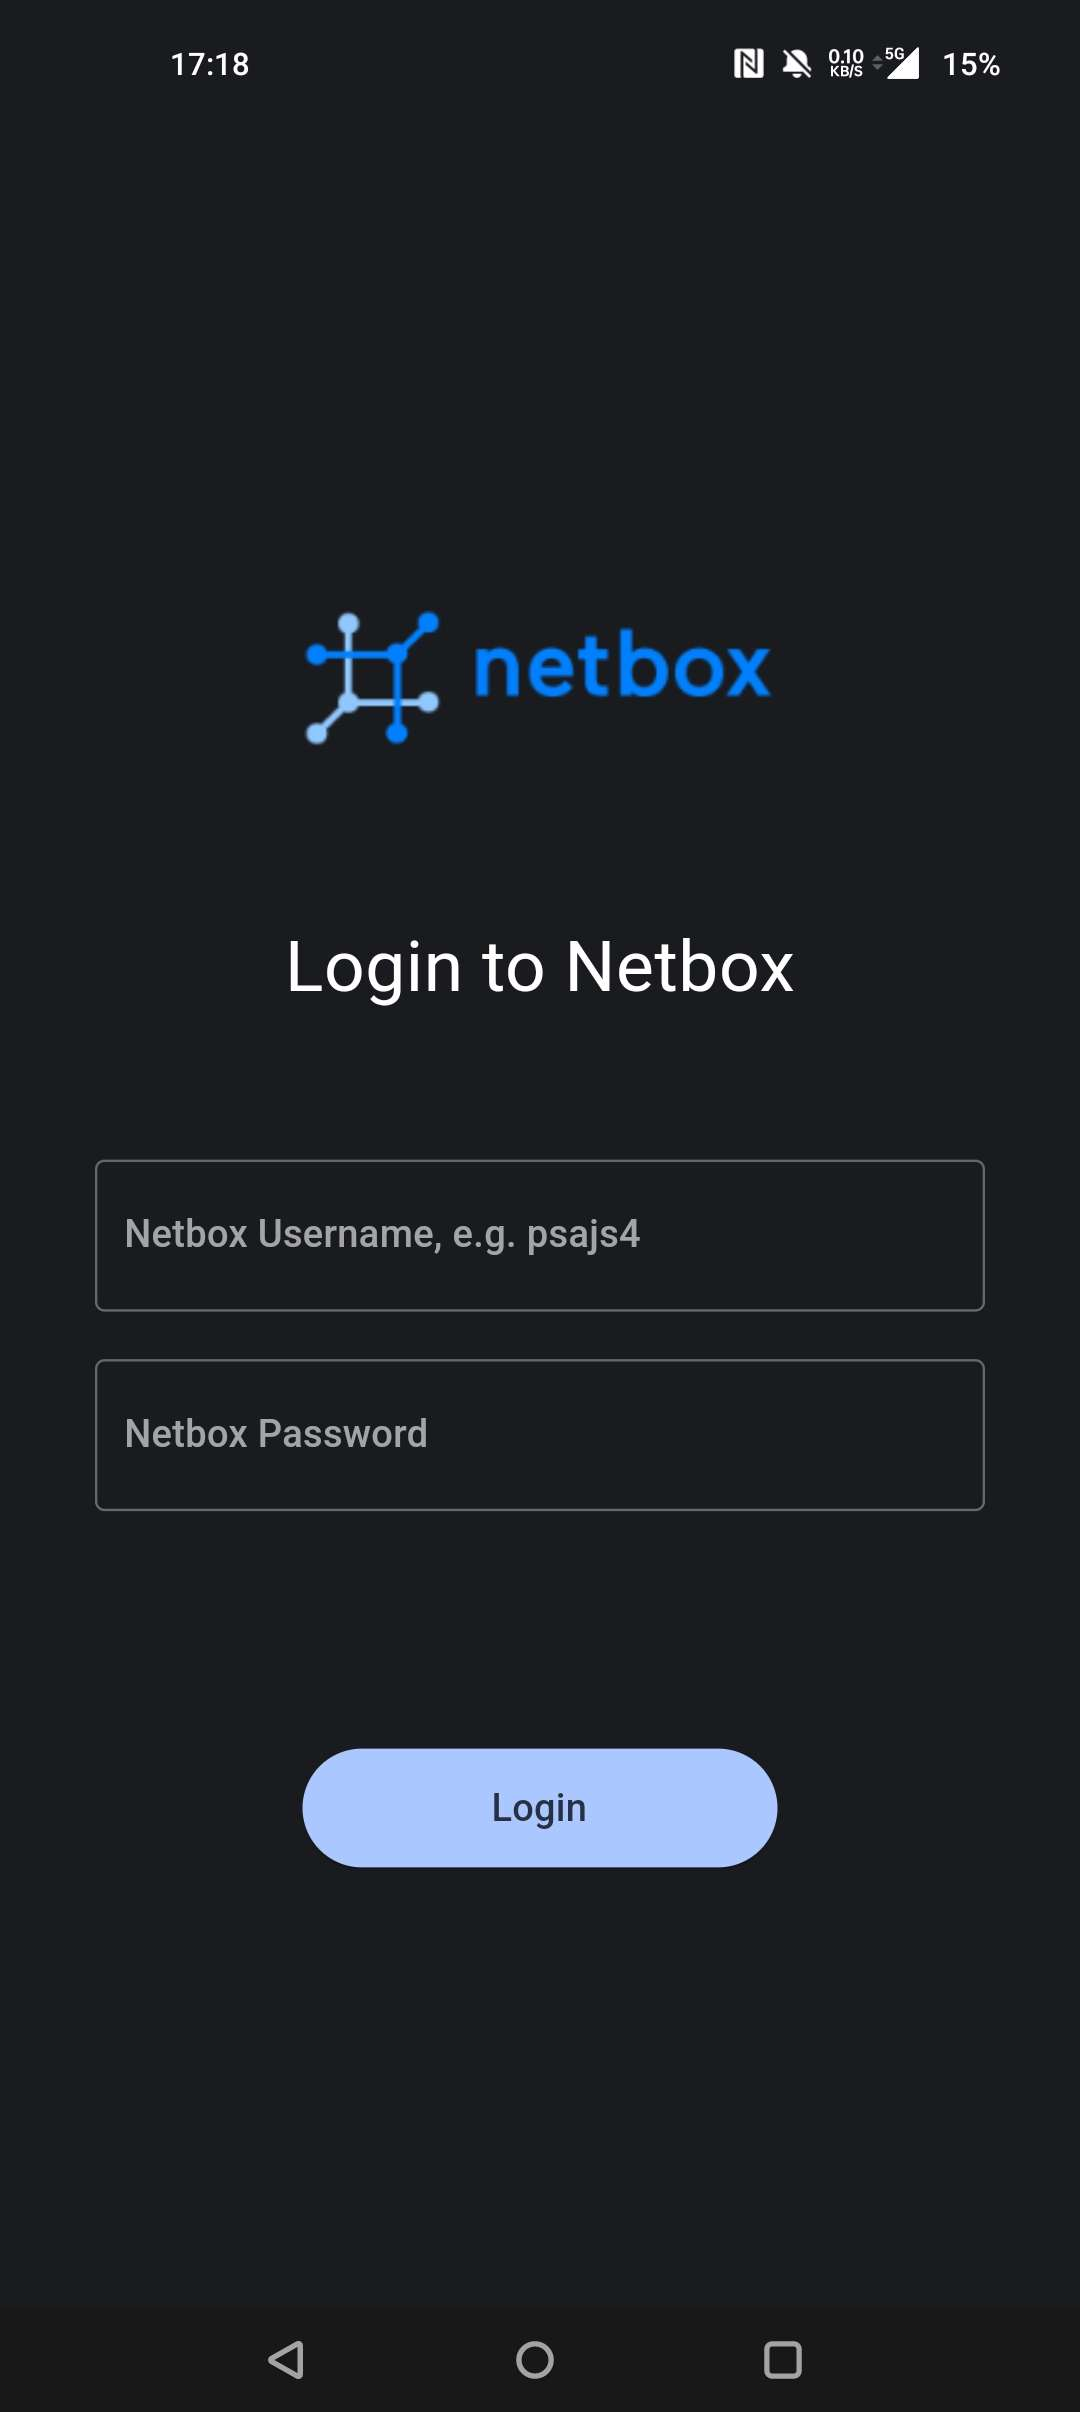
\includegraphics[width=2.5cm]{images/login.png} }}%
    \qquad
    \subfloat[\centering Add Connection Page]{{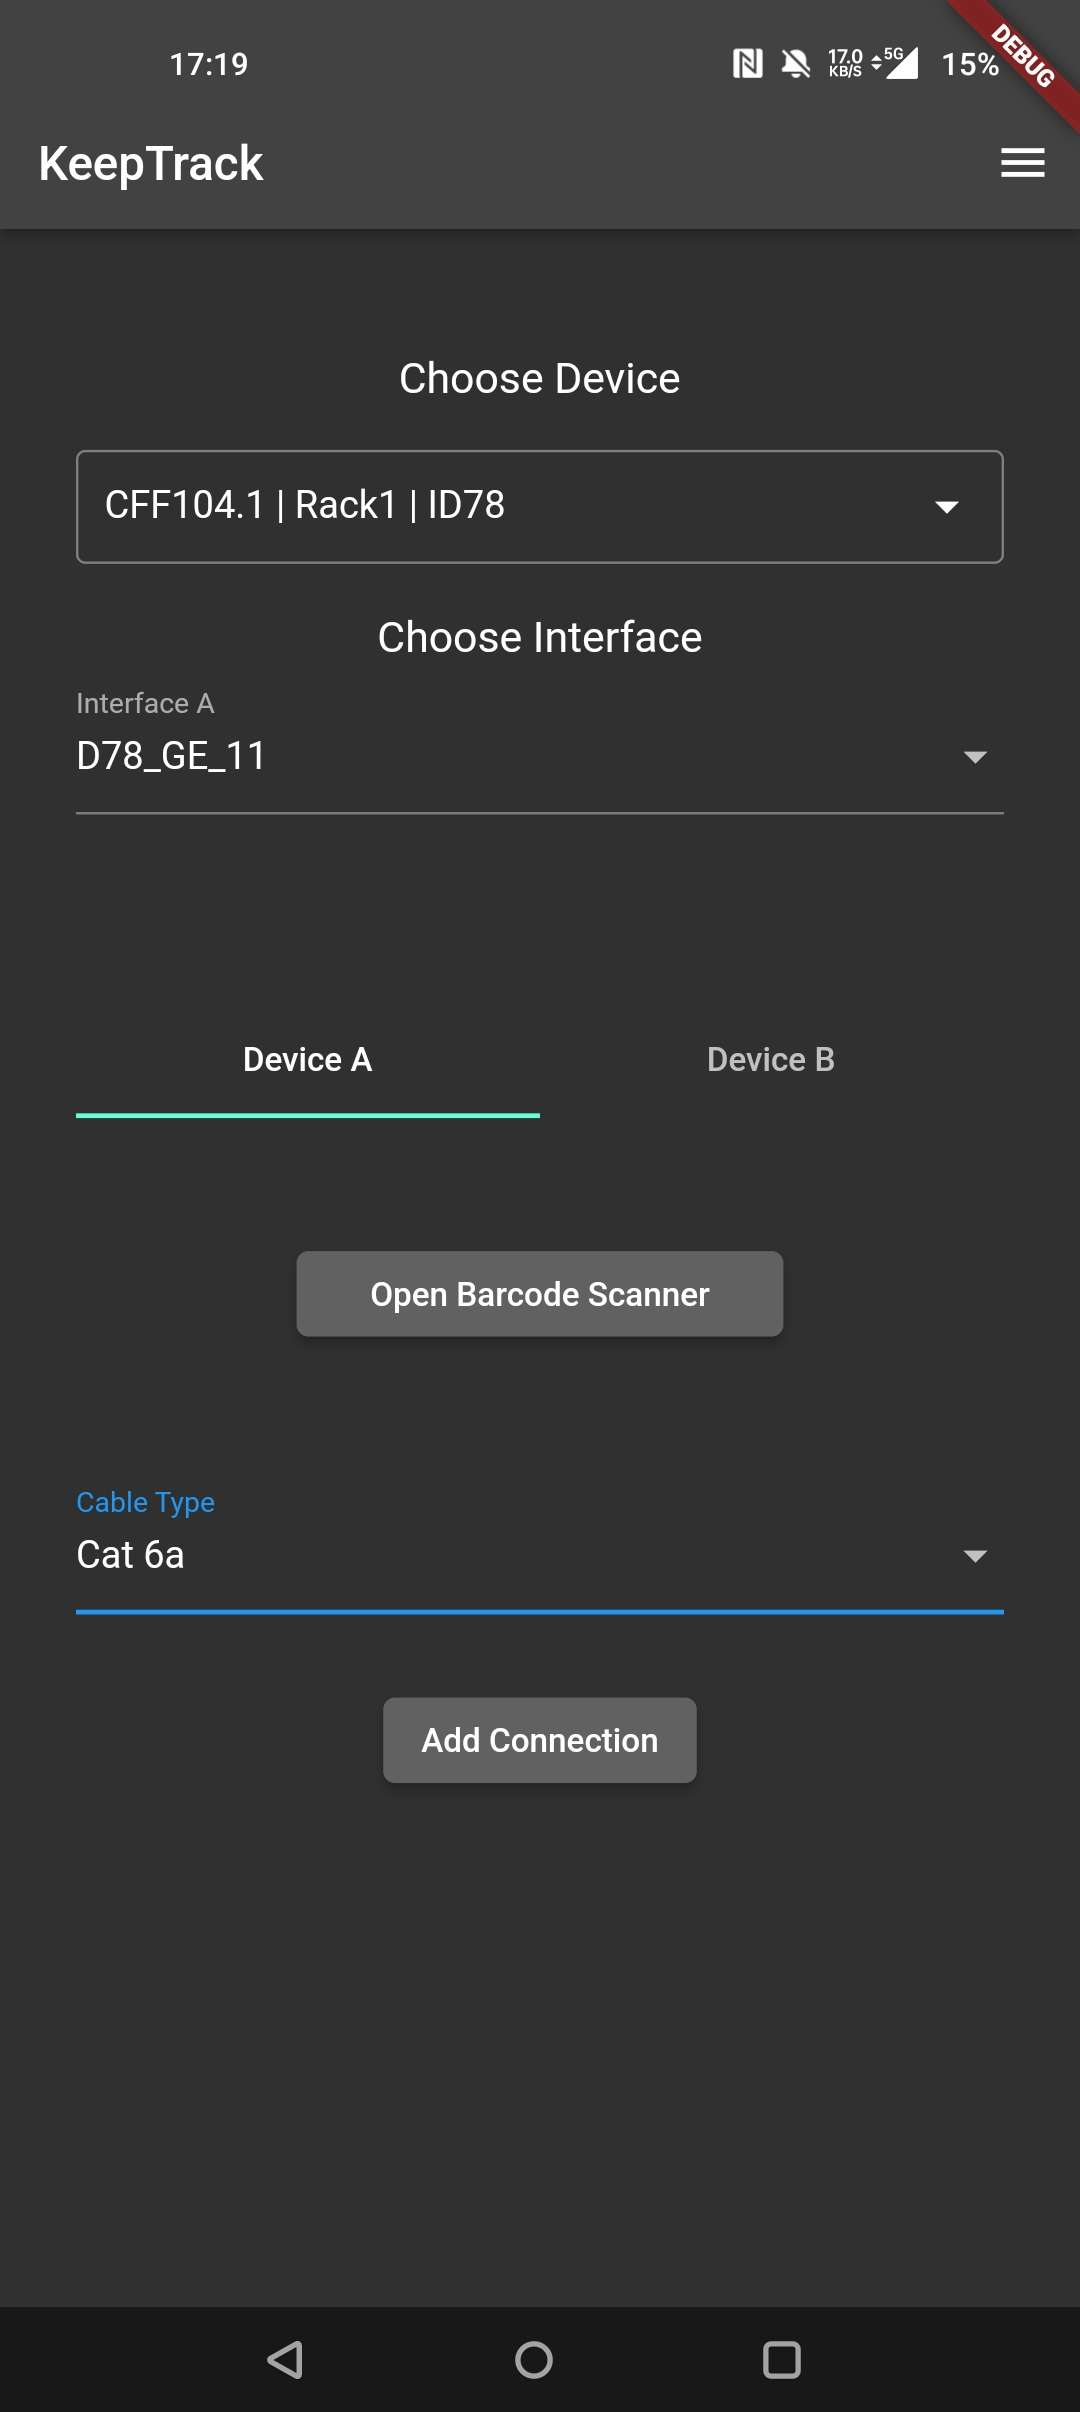
\includegraphics[width=2.5cm]{images/addcon.png} }}%
    \qquad
    \subfloat[\centering Device Search]{{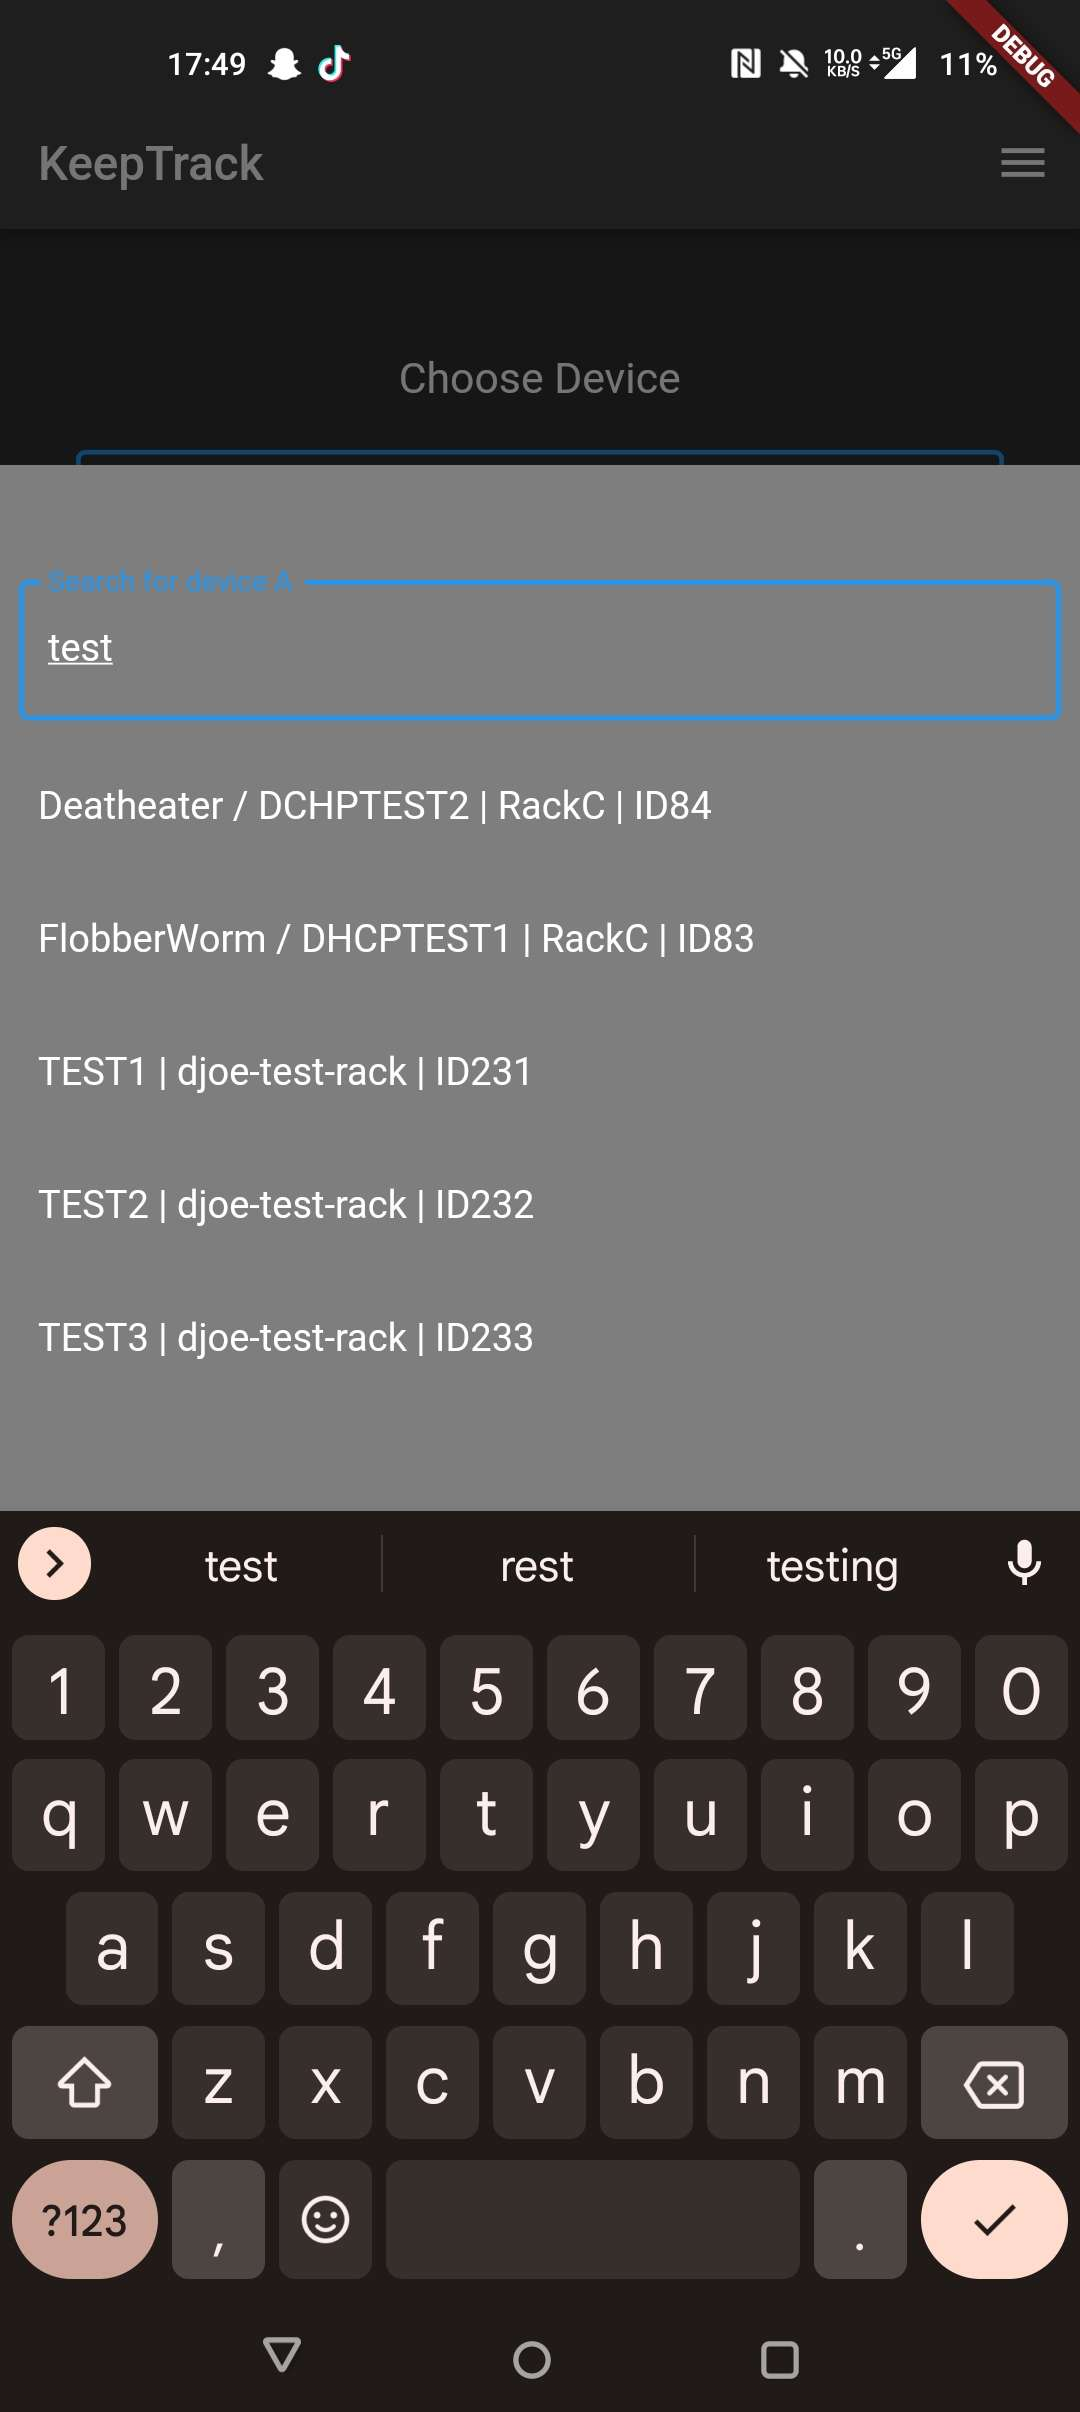
\includegraphics[width=2.5cm]
    {images/search.png} }}%
    \caption{Screenshots of the current Keeptrack UI}%
    \label{fig:currentUIScreenshots}%
\end{figure}


\section{Progress}
\label{sec:progress}
The following section will outline the progress made on the project, and the challenges faced. Further, it describes the future work plan and adjustments to milestones. 
\subsection{Projection Management}
\label{sec:project_management}

Whilst the project is still in its early stages, there has been some good progress made, though less so than initially planned. This is due to several factors. Firstly, I hadn't assigned enough weekly time to work on the project, which has led to slower progress overall. Secondly, I hadn't accounted for interviewee availability, which led to a delay in the interviews and therefore the creation of the high-fidelity prototypes. However, I have been able to make progress on the technical side of the project, which has allowed me to create a foundation for the UI and the core logic of the app. I am satisfied with the technical progress made and I believe that with the core foundations now in place, technical progress can be completed more quickly.

\pagebreak

I also didn't expect that the literature review would take as long as it did, or more specifically for this project - finding similar applications along with technical and HCI-based papers. Finding applications that had easily accessible trials posed a harder challenge than I had anticipated. But I believe that the similar work I have found has given me a better insight into a mixture of HCI and technical aspects of the project. Though, I struggled to find HCI-focused papers that were related to the scenario posed, e.g. encumbered use of a mobile device. 

On a positive note, the interviews brought up some interesting points that I hadn't considered before. For example, an inbuilt SSH terminal, and augmented reality features, but also increasing the scope of the project to include other rooms. Whilst some of the ideas risen can be achieved easily, others will require more time and research. However, I believe that the interviews have been a success and have given me a better understanding of the stakeholders and their needs.

With the delay and change in some aspects of the project, I have had to re-evaluate aspects of the new work plan. Shifting milestones along and re-assigning tasks to more/less work. I believe that in the work plan I hadn't accounted for a large enough research period, i.e. finding similar work, but now that this has been completed, I can focus on getting on with the technical work.

Comparing the initial Gantt chart, seen in appendix \ref{sec:init_gantt_charts}, to the updated Gantt chart, appendix \ref{sec:updated_gantt_charts}, it has become apparent that I have had to shift the milestones along. But this mainly filled most of the run-over time I had assigned in the initial plan. But even with these delays, I am confident that I can complete the project within the time frame given.

During weekly meetings with the project supervisor, we discussed the progress made and the work that needs to be completed. To keep track of the discussions, a document was maintained. Each meeting I would write up a summary of topics I wanted to discuss, and then during the meeting add notes to each section. Then following the meeting, I would review a Trello board (See appendix \ref{sec:trello_board}) to see what tasks I had completed and what tasks I needed to complete. Though, initially, I didn't assign dates to each task this was changed quickly after failing to achieve tasks in coordination with the work plan. Additionally, each task is also colour coded based on work type. 

\subsection{Contributions and Reflections}
\label{sec:contributions}
The primary contributions I have made to the project so far are the literature review, interviews and technical work done to date. From this work, I'll be able to create a set of high-fidelity prototypes and start creating a Minimal Viable Product (MVP) soon after. Although, I am aware that I have somewhat fallen behind on the project. I estimate this to only be a week or two behind, but with the reshuffling of the work plan, and the time set aside for run-over, I am confident that I can complete the project within the time frame given.

Overall I am happy with the progress made so far. Initially, whilst I had a good idea of what the app needed to be, following the work done I have a better understanding of what will make the app useful. Additionally, I have also learnt that there is a significant lacking in the market for a product like this. 


Notably, I think it is important that I reach out to external stakeholders, outside of the university, to get a better understanding of the market and what is needed. It is possible that more ideas will arise from this and that the project will not be limited to what RST needs. 

I think that with the next steps of the project it is important that I establish a more constant workflow, rather than the bursts of work I have carried out so far. I think that this will create more iterative progress and can prompt more user feedback. Notably, I think that there is a bigger risk of feature creep than I expected and I think I will need to pay more attention to this moving forward.

\subsubsection{Laws, Social, Ethical and Professional Issues}
\label{sec:computer_laws}
As this project intends to be open source under the Mozilla Public License Version 2.0 I foresee no implications for intellectual property. It is currently and will be publicly available via Github \cite{keeptrackgithub}. Although, it is possible the work may be exploited for commercial gain but is dependent on the success of the project and the possibility to be implemented externally.

Due to the project involving human participants, I have had to complete the full ethics form, "CS REC 1", and have received approval from relevant parties. Further as set out by the Research ethics guidelines \cite{ethicsguidelines}, I have completed the Data Management Plan (DMP) form. This form outlines how I will store and manage the data collected during the interviews. Each interviewee was given a consent form to sign, outlining the purpose of the interview and the data collection. The interviewees have also been given the option to opt-out of the interview at any point.

Additionally, there are notices regarding the Data Protection Act (2018). The  data collected will be stored on a password-protected computer and will be deleted after the project has been completed.

I believe that from a broader perspective, this project will not have significant implications for society. Though, I do believe that it will have a positive impact on the RST team and the wider system administrator community. I believe with the project being open source and with a focus on HCI, it will be accessible to a wide range of people. Further giving DCIM software another platform to be accessed, I believe that will be a positive step towards the future of DCIM software and data centre management.

\pagebreak

% Bibliography
\bibliographystyle{ieeetr}
\bibliography{citation} 

% Appendix
\appendix
\section{Appendix}
\label{sec:appendix}
\subsection{Trello Board}
\label{sec:trello_board}
\begin{figure}[H]
    \centering
    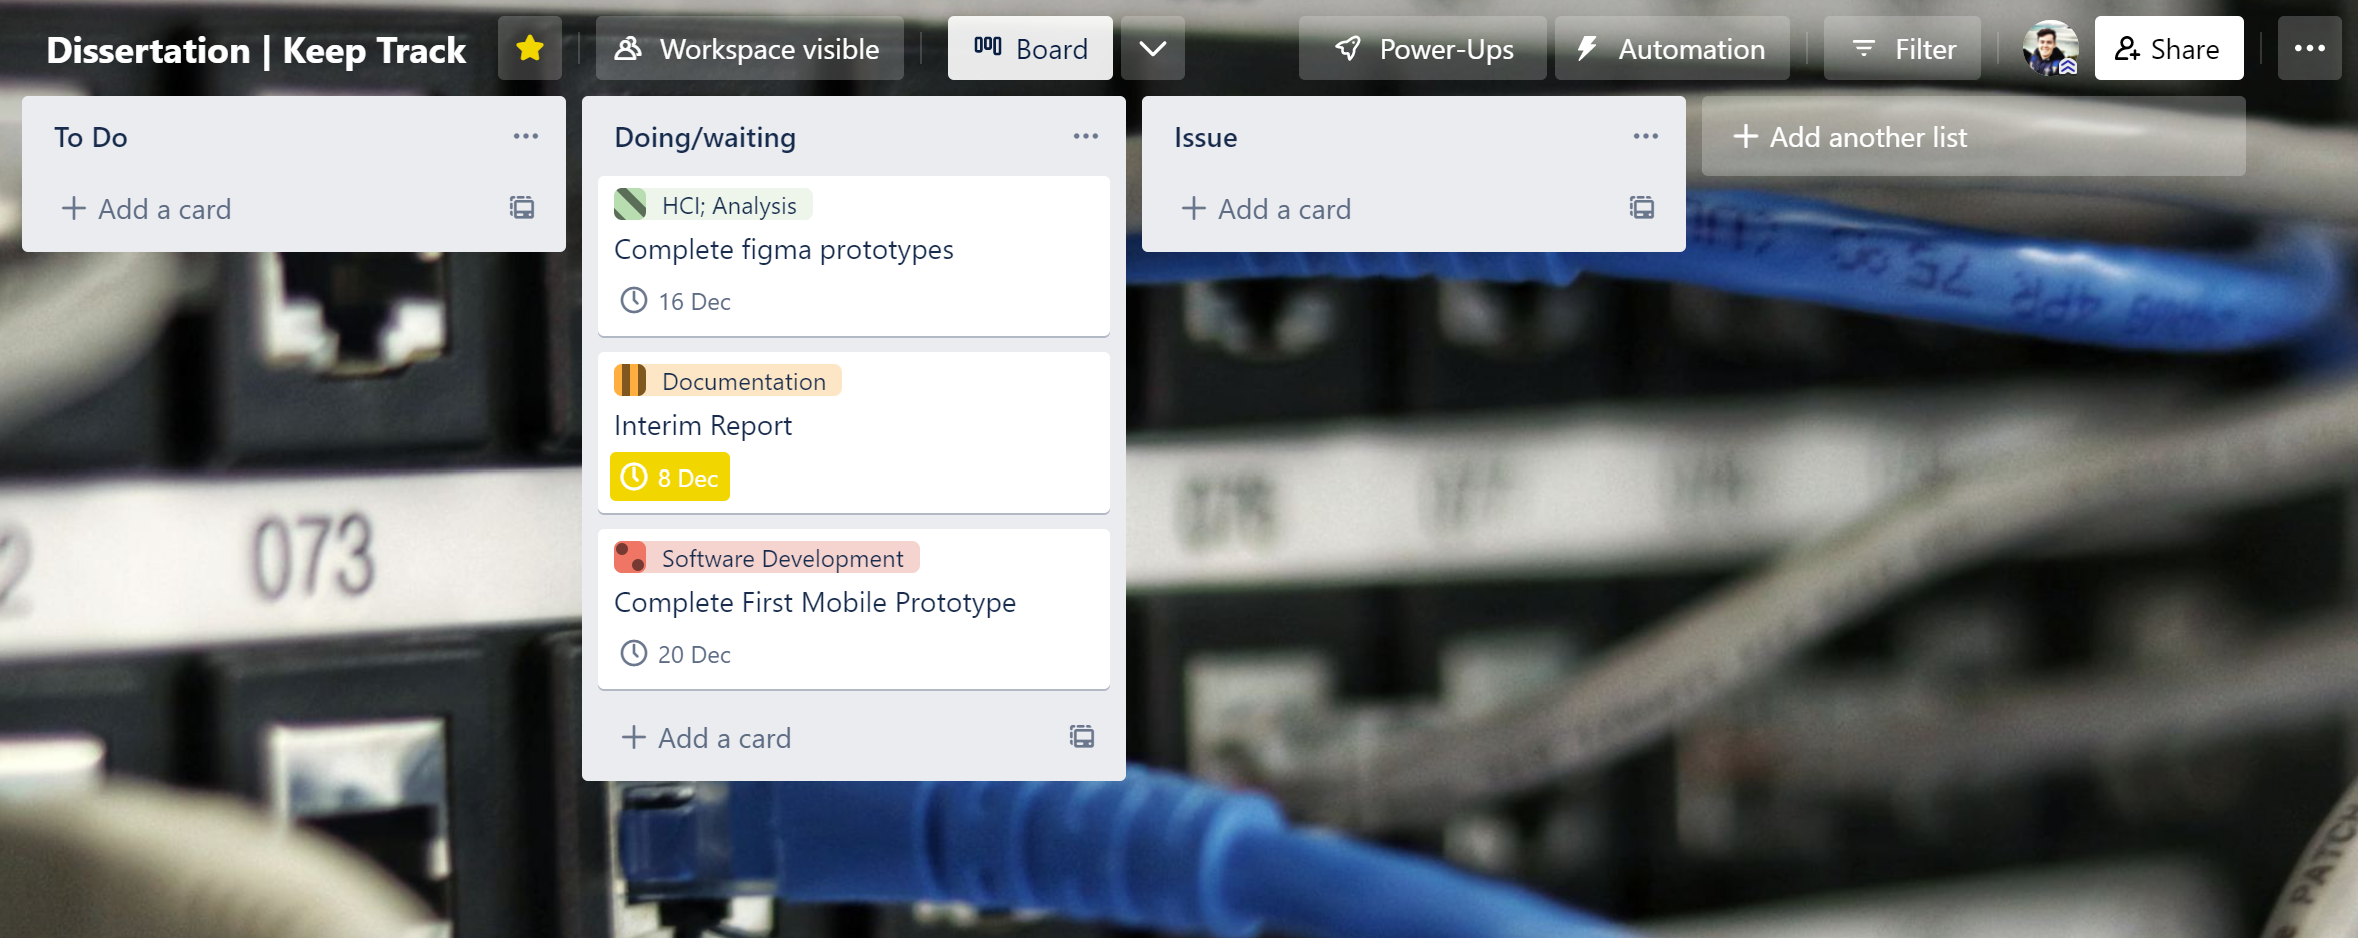
\includegraphics[width=.75\textwidth]{images/trello-board.png}
\end{figure}   

\subsection{Initial Gantt Chart}
\label{sec:init_gantt_charts}
\begin{figure}[H]
    \centering
    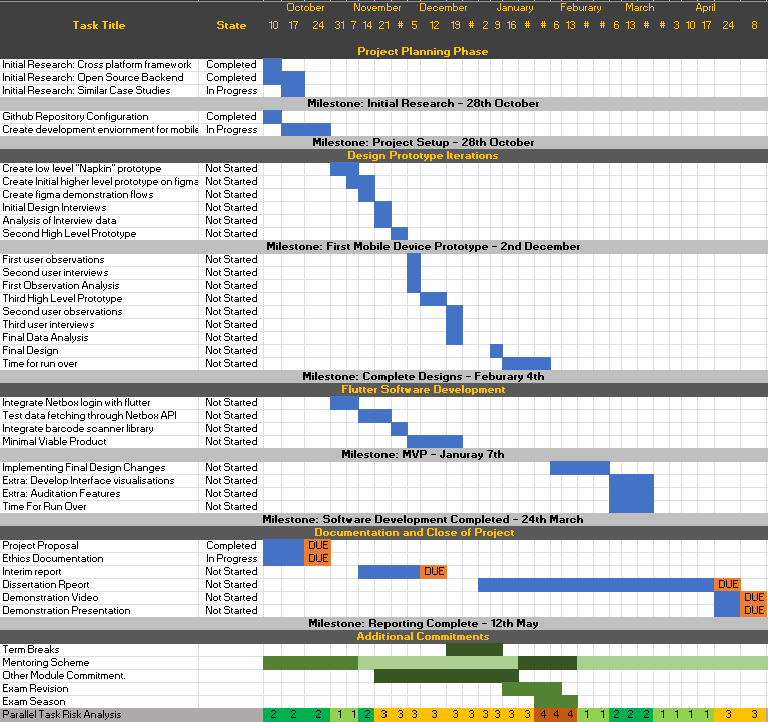
\includegraphics[width=0.75\textwidth]{images/keeptrack-gantt-initial.png}
    \label{fig:initialworkplan}
\end{figure}

\subsection{Updated Gantt Chart}
\label{sec:updated_gantt_charts}

\begin{figure}[H]
    \centering
    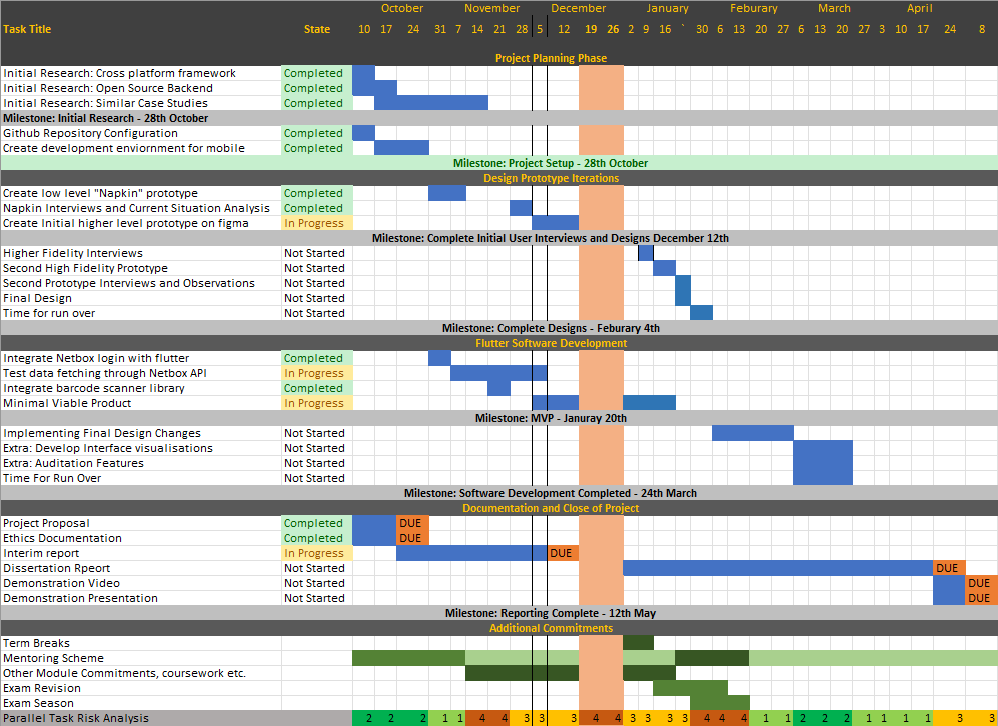
\includegraphics[width=0.85\textwidth]{images/keeptrack-gantt-interim.png}
    \label{fig:updatedworkplan}
\end{figure}


% Document End
\end{document} 